%%%%%%%%%%%%%%%%%%%%%%%%%%%%%%%%%%%%%%%%%%%%%%%%%%%%%%%%%%%%%%%%%%%%%
%% This is a (brief) model paper using the achemso class
%% The document class accepts keyval options, which should include
%% the target journal and optionally the manuscript type.
%%%%%%%%%%%%%%%%%%%%%%%%%%%%%%%%%%%%%%%%%%%%%%%%%%%%%%%%%%%%%%%%%%%%%

\documentclass[a4paper, 12pt, openany]{book}
\usepackage[style = chem-acs, autocite = superscript]{biblatex}
\bibliography{references.bib}
\renewcommand{\baselinestretch}{1.5}
\usepackage[version=3]{mhchem} % Formula subscripts using \ce{}
\usepackage{chemnum}

\usepackage{multirow}
\usepackage{textgreek}
\usepackage{textcomp}
\usepackage{setspace}
\usepackage{afterpage}
\usepackage{caption}
\usepackage{floatrow}
\usepackage{gensymb}
\usepackage{mathtools}
\usepackage[outdir=./]{epstopdf}

\usepackage[bottom=2cm,top=2cm, right=2cm, left=2cm, headsep=5pt]{geometry}


\usepackage{amsmath}


\captionsetup{justification=raggedright,singlelinecheck=false}

\usepackage[labelfont=bf]{caption}
\usepackage{makecell}

\usepackage{dblfloatfix}
\usepackage{framed}

\usepackage{tabularx} % for 'tabularx' environment
\usepackage{array}

\usepackage[hyperref = true]{acro}

\usepackage{tocloft}
\cftsetrmarg{7em}% Default is 2.55em

% \acsetup{hyperref=true}

\usepackage{enumitem}

\usepackage{multicol}
\usepackage{graphicx}
\usepackage{subcaption}

% glossary
\usepackage{hyperref}


\hypersetup{
    colorlinks,
    citecolor=black,
    filecolor=black,
    linkcolor=black,
    urlcolor=black
}

\usepackage{fancyhdr}
\pagestyle{fancy}

\renewcommand{\headrulewidth}{.01em} % Headline 
\renewcommand{\chaptermark}[1]{\markboth{\thechapter{\hspace{0.5cm}}\ #1}{}}
\fancyhead[L]{\nouppercase{\leftmark}}
\fancyhead[R]{}

\usepackage[T1]{fontenc}
\usepackage{titlesec, blindtext, color}
\definecolor{gray75}{gray}{0.75}
\newcommand{\hsp}{\hspace{10pt}}
\titleformat{\chapter}[hang]{\Huge\bfseries\raggedright}{\thechapter\hsp\textcolor{gray75}{|}\hsp}{0pt}{\Huge\bfseries}


\titlespacing{\chapter}{5pt}{*4}{*1.5}
\titlespacing{\section}{0pt}{*4}{*1.5}
\titlespacing{\subsection}{0pt}{*4}{*1.5}
\titlespacing{\subsubsection}{-5pt}{*4}{*1.5}

%%%%%%%%%%%%%%%%%%%%%%%%%%%%%%%%%%%%%%%%%%%%%%%%%%%%%%%%%%%%%%%%%%%%%
%% If issues arise when submitting your manuscript, you may want to
%% un-comment the next line.  This provides information on the
%% version of every file you have used.
%%%%%%%%%%%%%%%%%%%%%%%%%%%%%%%%%%%%%%%%%%%%%%%%%%%%%%%%%%%%%%%%%%%%%
%%\listfiles

%%%%%%%%%%%%%%%%%%%%%%%%%%%%%%%%%%%%%%%%%%%%%%%%%%%%%%%%%%%%%%%%%%%%%
%% Place any additional macros here.  Please use \newcommand* where
%% possible, and avoid layout-changing macros (which are not used
%% when typesetting).
%%%%%%%%%%%%%%%%%%%%%%%%%%%%%%%%%%%%%%%%%%%%%%%%%%%%%%%%%%%%%%%%%%%%%
\newcommand*\mycommand[1]{\texttt{\emph{#1}}}

\DeclareAcronym{PDB}{
    short = PDB,
    long = Protein Data Bank
}

\DeclareAcronym{GAG}{
    short = GAG ,
    long = glycosaminoglycan
}

\DeclareAcronym{QM}{
    short = QM ,
    long = quantum mechanics
}

\DeclareAcronym{MD}{
    short = MD ,
    long = molecular dynamics
}

\DeclareAcronym{VC}{
    short = VC ,
    long = Vina--Carb
}

\DeclareAcronym{ADV}{
    short = ADV ,
    long = Autodock Vina
}

\DeclareAcronym{RMSD}{
    short = RMSD ,
    long = root-mean-squared deviation
}


\newcommand{\squeezeup}{\vspace{-2.5mm}}


\begin{document}

\begin{titlepage}
\begin{center}

\vspace*{3cm}
\renewcommand{\thefootnote}{\fnsymbol{footnote}}
\pagenumbering{gobble}


\includegraphics[]{Pictures/PNGLogo.png}
\vspace{0.2cm}


\vspace{2cm}
\textbf{\LARGE{Development of Computational Tools for the Rational Design of Glycosaminoglycan Mimetics}} \\

by Eric David Boittier \\

\vspace{0.5cm}

Supervisor: Associate Professor Vito Ferro
\\
Co-supervisor: Doctor Neha S. Gandhi
\\
\vspace{3cm}
\textit{A	Research report submitted for	the	degree	of	Bachelor of	Advanced Science	(Honours)	at
\\ The	University	of	Queensland	in	May	2018}
\\School	of	Chemistry	and	Molecular	Biosciences
\end{center}
\end{titlepage}


\newpage

% \addtolength{\topmargin}{-3in}
% \addtolength{\textheight}{-3in}

% 	\addtolength{\textwidth}{1in}

% 	\addtolength{\topmargin}{-.5in}
% 	\addtolength{\textheight}{1.75in}
	


\begin{footnotesize}
\noindent
\textbf{Declaration by the author}\\
This	research	report	is	composed	of	my	original	work,	and	contains	no	material	previously	published	or	written	by	another	person	except	where	due	reference	has	been	made in	the	text. I	have clearly	stated the	contribution by	others	to jointly-authored works that I have included in	my	report.\\
\indent I have clearly	stated the	contribution of	others	to	my	research report	as	a	whole, including statistical	assistance,	survey	design,	data analysis,	significant	technical	procedures,	professional editorial advice,	and	any other original research work used	or reported in	my	report.	The	content	of	my	report	is	the	result	of	work I	have carried	out	since the	
commencement of	my	honours	research project	and	does not	include	a	substantial	part	of work that has	been submitted to qualify	for	the	award	of	any	other degree	or	diploma	in	any	university or other tertiary institution. I have clearly	stated	which parts of my	research report,	if any, have	been	submitted	to	qualify	for	another	award.\\
\indent I	acknowledge	that	copyright	of	all	material	contained	in	my	research report	resides	with the	copyright	holder(s)	of	that	material.
\\
\\
\textbf{Statement	of	Contributions	to	Jointly	Authored Works	Contained	in	the	Research	Report}
\\
No jointly-authored	works.
\\
\\
\textbf{Statement	of	Contributions	by	Others	to	the	Research	Report	as	a	Whole}
\\
No	contributions	by	others.	
\\
\\
\textbf{Statement of Parts of the Research Report or Submitted to Qualify for the Award of Another Degree}
\\
None
\\
\\
\textbf{Published	Works	by	the	Author	Incorporated	into	the	Research}\\
None
\\
\\
\textbf{Additional	Published	Works	by	the	Author	Relevant to	the	Research Report	or	but	not	Forming Part of it}\\	
Pathway Bifurcation in the (4 + 3)/(5 + 2)-Cycloaddition of Butadiene and Oxidopyrylium Ylides: The Significance of Molecular Orbital Isosymmetry
Jed M. Burns and Eric D. Boittier
\textit{J. Org. Chem.}
DOI: 10.1021/acs.joc.8b03236
\\
\\
\textbf{Signature	of	Author: \rule{4cm}{0.4pt}       Date: \rule{4cm}{0.4pt}}
\\
\\
\textbf{Principal	Supervisor	Agreement}
\\
I have read	the	final report and agree	with the student's declaration.
\\
\\
\textbf{Signature	of	Principal	Supervisor: \rule{4cm}{0.4pt}        Date: \rule{4cm}{0.4pt}}

\end{footnotesize}
\newpage
\pagenumbering{roman} 
\chapter*{Acknowledgements}
\addcontentsline{toc}{chapter}{Acknowledgements}

\newpage

%%%%%%%%%%%%%%%%%%%%%%%%%%%%%%%%%%%%%%%%%%%%%%%%%%%%%%%%%%%%%%%%%%%%%
%% The manuscript does not need to include \maketitle, which is
%% executed automatically.  The document should begin with an
%% abstract, if appropriate.  If one is given and should not be, the
%% contents will be gobbled.
%%%%%%%%%%%%%%%%%%%%%%%%%%%%%%%%%%%%%%%%%%%%%%%%%%%%%%%%%%%%%%%%%%%%%



{\setstretch{1.2} 
\renewcommand{\contentsname}{Table of Contents}
% \renewcommand{\thesubfigure}{\Alph{subfigure}}

\tableofcontents
\listoffigures
\addcontentsline{toc}{chapter}{List of Figures}
\listoftables
\addcontentsline{toc}{chapter}{List of Tables}
\chapter*{Acronyms}
\addcontentsline{toc}{chapter}{Acronyms}
\begin{multicols}{2}
\setstretch{1}
\DeclareInstance{acro-title}{empty}{sectioning}{name-format =}
\printacronyms[heading=none]

\end{multicols}
}


%%%%%%%%%%%%%%%%%%%%%%%%%%%%%%%%%%%%%%%%%%%%%%%%%%%%%%%%%%%%%%%%%%%%%
%% Start the main part of the manuscript here.
%%%%%%%%%%%%%%%%%%%%%%%%%%%%%%%%%%%%%%%%%%%%%%%%%%%%%%%%%%%%%%%%%%%%%
\pagebreak
\pagenumbering{arabic} 

\chapter*{Abstract}
\addcontentsline{toc}{chapter}{Abstract}

\newpage

\chapter{Computer Aided Drug Design \& Glycosaminoglycans}
\section{Adrift in Chemical Space}

\section{Glycosaminoglycans in Biology and Medicine}
\subsection{Structure and Function}
\subsection{Case Study 1: Antithrombin and Fondarinux}
\subsection{Case Study 2: Heparanase and PG545}
\newpage

\section{Computational Chemistry (in a Nutshell)}
% \begin{figure}[h]
%     \centering
%     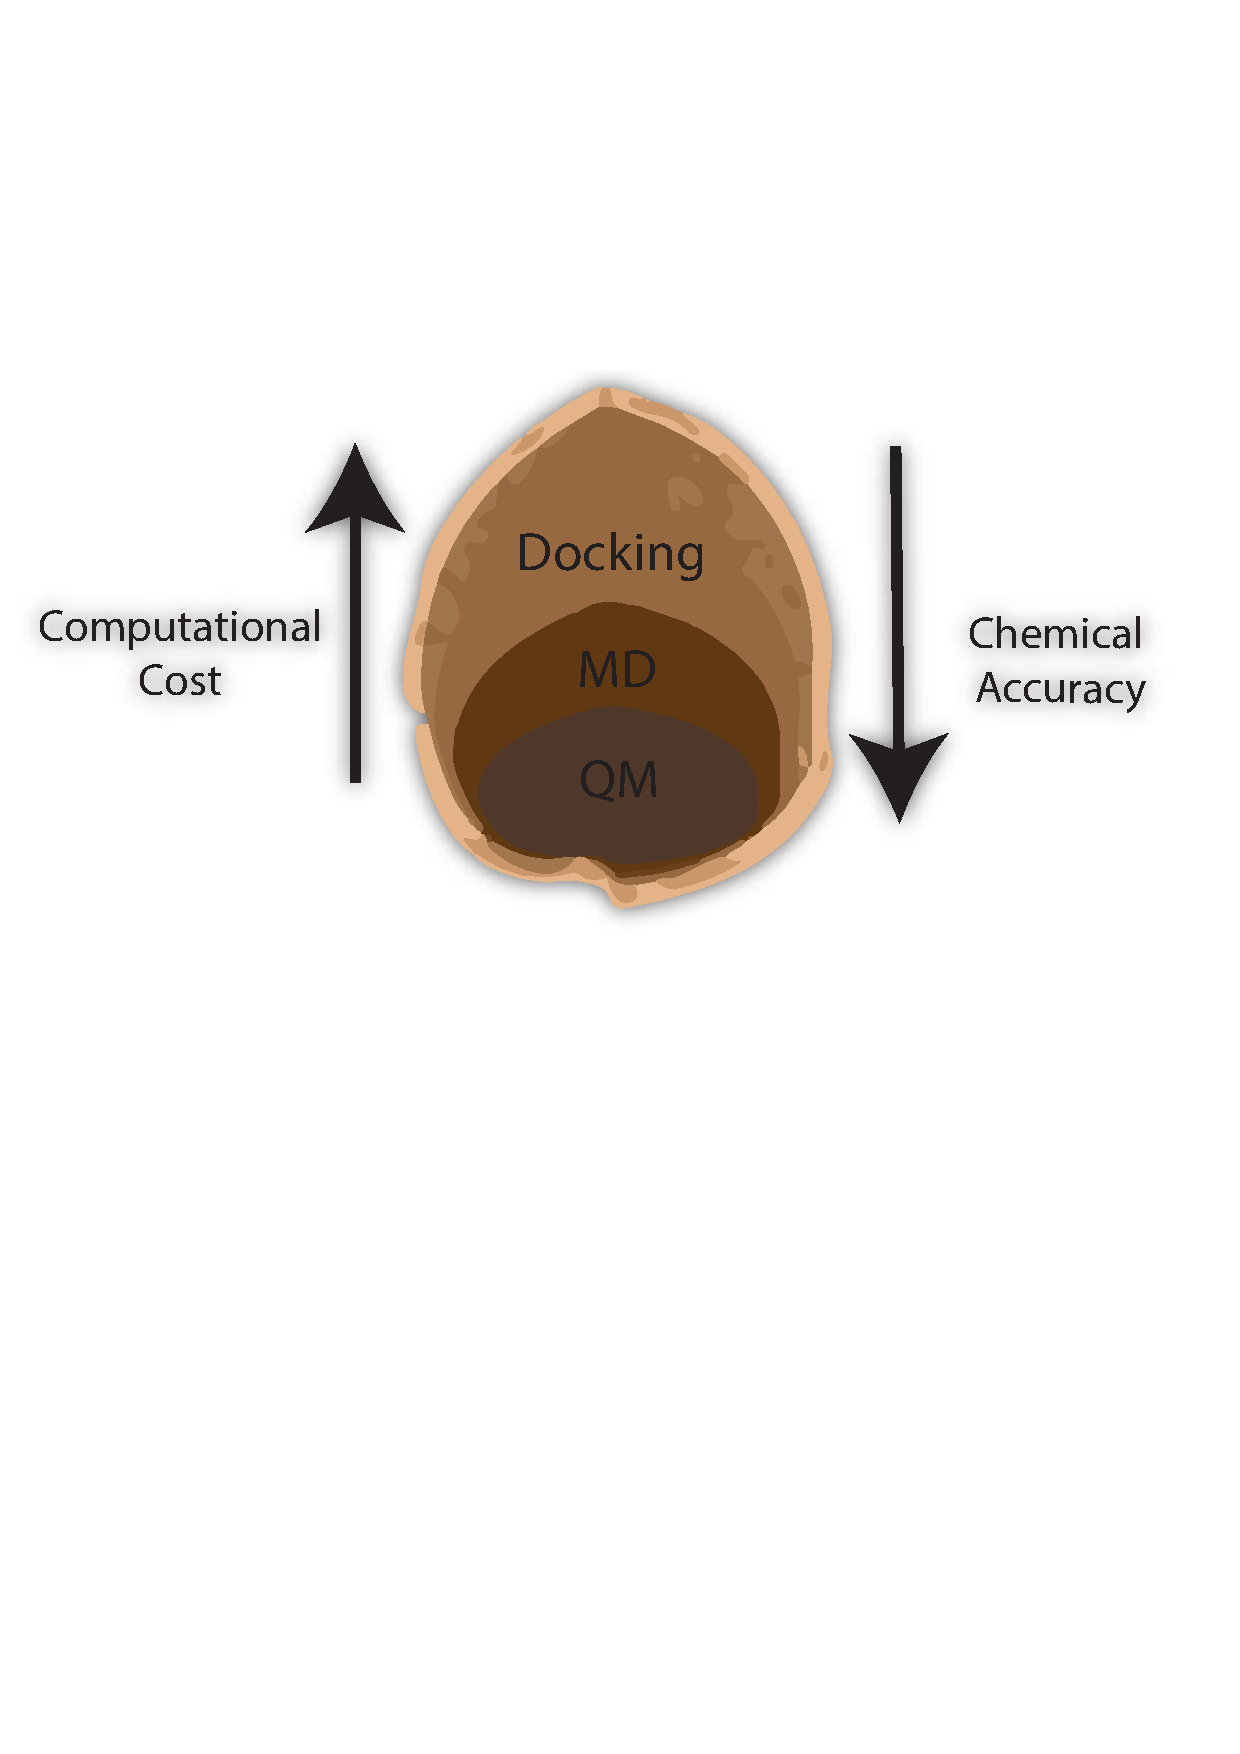
\includegraphics[width=8cm]{Figures/Intro/computational_chemistry_in_a_nutshell.pdf}
%     \caption{A suggested paradigm for scientific programming.}
%     \label{fig:my_label}
% \end{figure}



\chapter{Methods Development in Protein-Ligand Docking}
\section{Theory}
\subsection{Search Functions}
\subsection{Scoring Functions}

\newpage
\section{Research Aims}
\noindent The aim of this project was to increase the accuracy of \textit{Vina-Carb} when predicting the structure of \acs{GAG}--Protein complexes by optimizing and developing new and existing scoring functions.
Alongside this aim, analyses of crystallographic data of \acs{GAG}--Protein complexes available in the \ac{PDB} were undertaken. 
Towards these goals, bespoke analytical tools necessary for this task were developed from new and existing software. This code was made entirely open-source. 
Tools from this code base considered particularly serviceable to the computational glycoscience community were hosted online as the Web-accessible server, \textit{GlycoTorch}, which aims to `shine a light on carbohydrate--protein interactions'.


\begin{figure}[h]
    \centering
    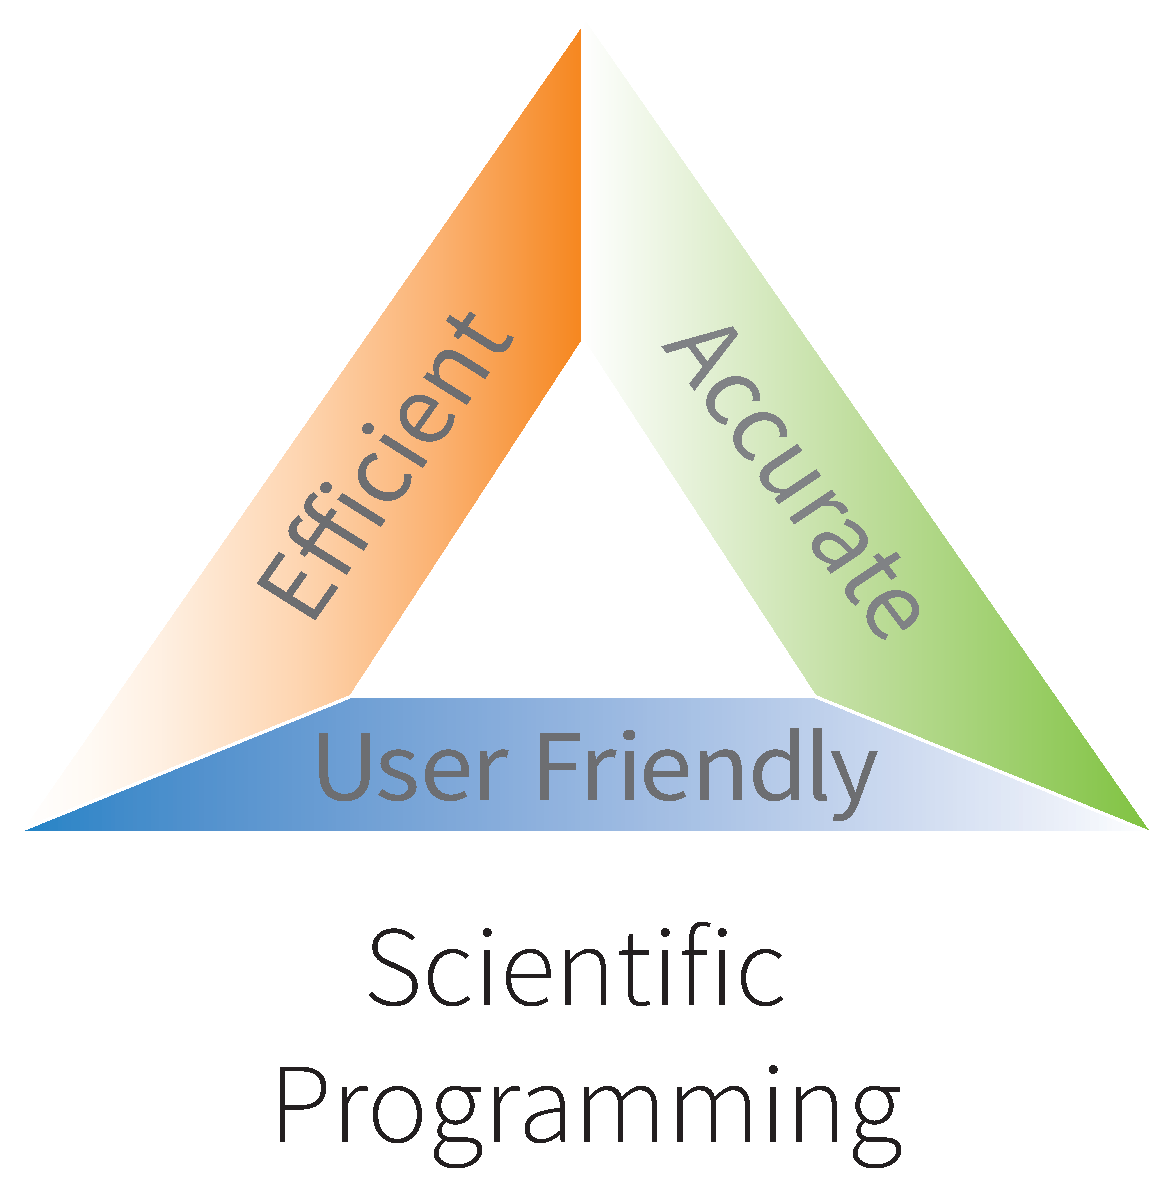
\includegraphics[width=6cm]{Figures/Intro/scientific_programming.eps}
    \caption{A suggested paradigm for scientific programming.}
    \label{fig:my_label}
\end{figure}



\chapter{Data Mining the Protein Data Bank for Glycosaminoglycan Interactions}

\section{Methods}

\subsection{The GAG70 Dataset: Creation and Curation}
Crystal structures in the \ac{PDB} containing glycosaminoglycans were identified. 
Previous work by Samsonov \textit{et. al.} provided 84 structures.\autocite{Samsonov2016}
From this dataset, the NMR structures (\ac{PDB} codes: 2LVZ, 1HPN) were discarded.
Structures from \ac{PDB} codes 5W1O and 5DNF were also 

\subsection{Carbohydrate Structure Analysis}

\noindent \textbf{Ring Conformations}\\
For analysis involving N--membered rings, relavent to fields such as crystallographic, NMR, \ac{MD} or \ac{QM} theoretical mechanistic studies for example, a formal method for describing ring conformations may be required. Historically, for rings composed of 6 atoms, six classical ring shapes are commonly assigned: chair (C), skew boat (S), boat (B), twist (T), envelope (E) and half boat (H). For sugars, depending on which atoms occupy the apex and/or bottom of the structure, the atom name is given with a superscript or subscript, respectively. This provides the basis of the 38 IUPAC standard ring conformations, which include, for example, the two most common and the typically low energy conformers, $^{4}C_{1}$ and $^{1}C_{4}$. These assignments are discrete and easy to visualize; however, they are idealized and unsuitable for describing dynamic structures, among other tasks. For this reason, a mathematically ``continuous'' description of ring conformations, ideally as system that can compliment the standard IUPAC descriptions, is also required. 
\\
\\
\noindent \textbf{Glycosidic Torsions}\\

\subsection{Intermolecular Interactions}

\begin{figure}
    \centering
    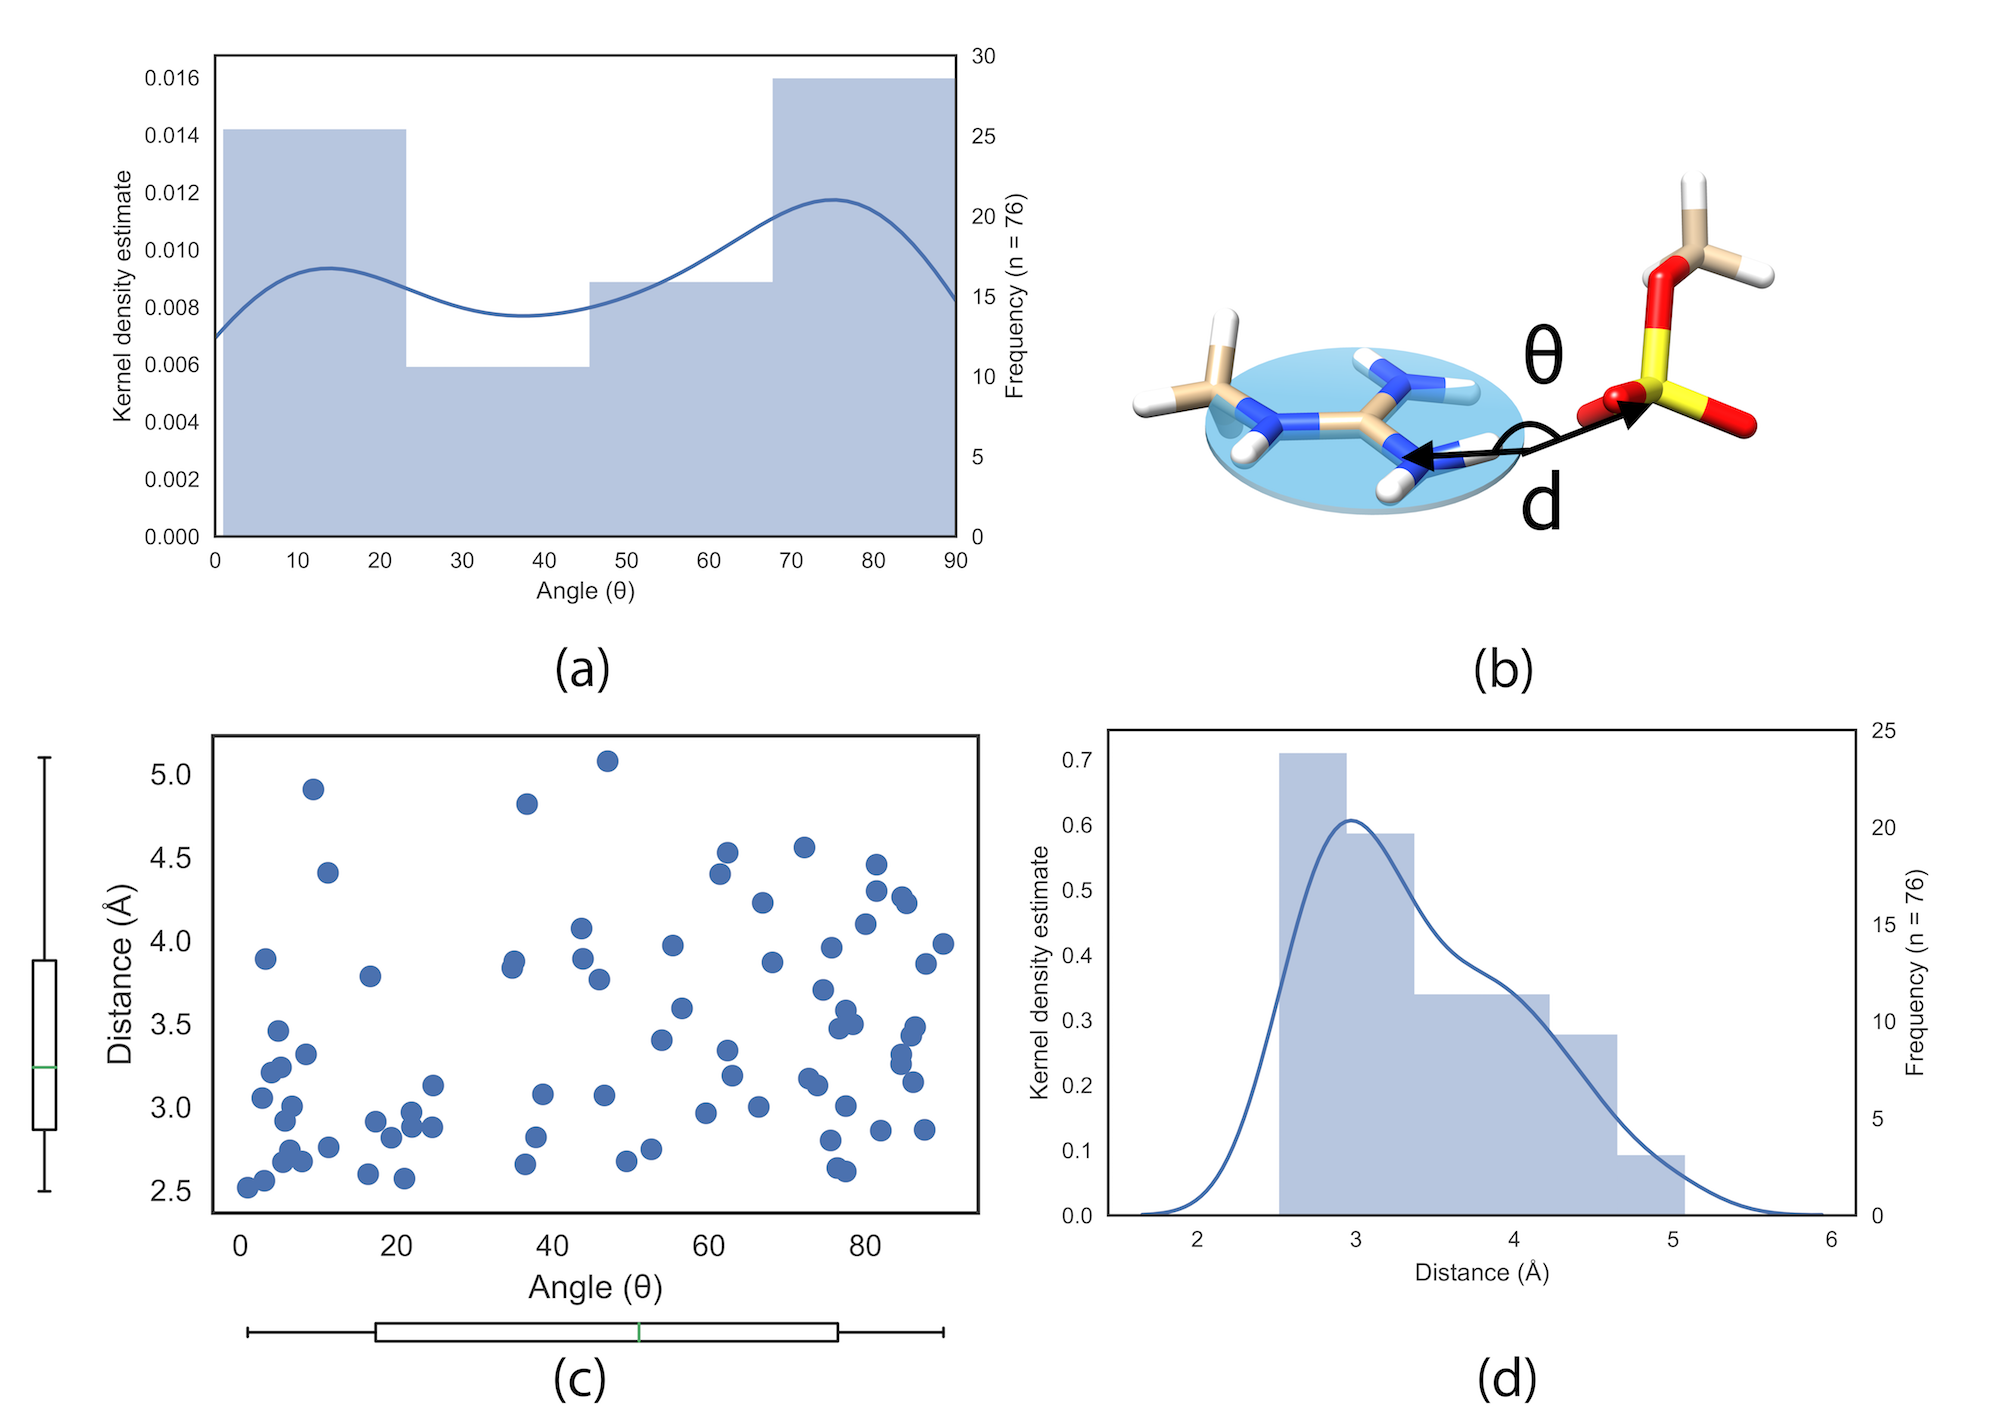
\includegraphics[width=9cm]{Figures/Datamining/arg_sulfate.png}
    \caption{
    % Distribution of (a) dihedral angles between arginine rings and sulfates and (d) \ce{S\bond{-}O- \bond{...}NH2+} distances shown using histogram and kernel density estimate. (b) Graphical representation of the interaction investigated. Distances and angles are shown. (c) Scatter plot of angles and distances suggests no clear relationship. The distribution of each variable is also shown using a boxplot.
    }
    \label{fig:my_label}
\end{figure}

\begin{figure}
    \centering
    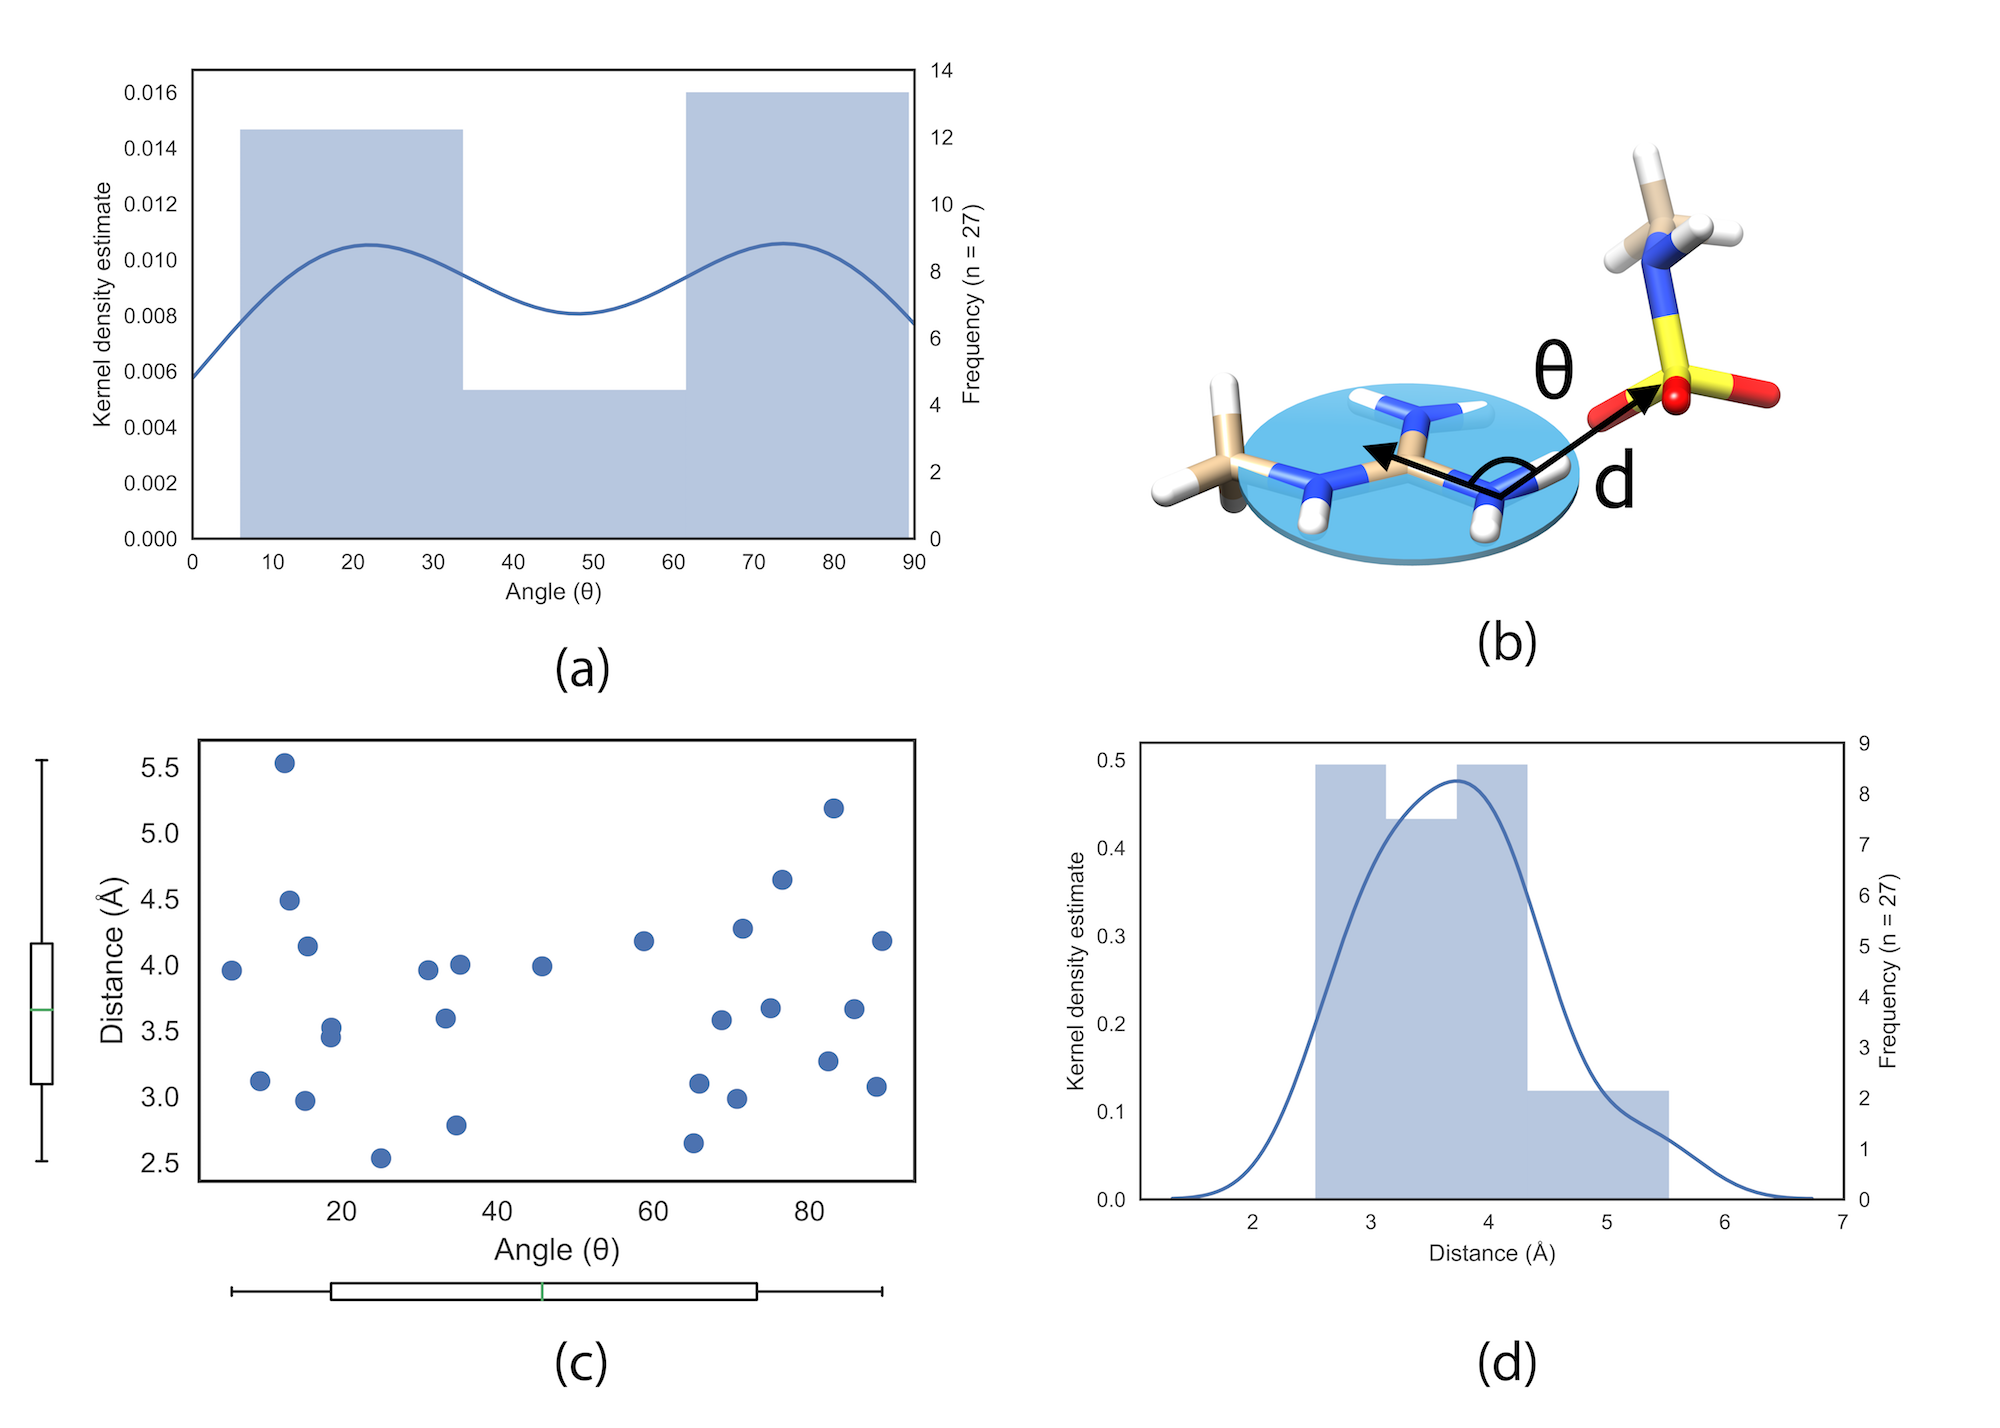
\includegraphics[width=9cm]{Figures/Datamining/arg_Nsulf.png}
    \caption{
    % Distribution of (a) dihedral angles between arginine rings and sulfates and (d) \ce{S\bond{-}O- \bond{...}NH2+} distances shown using histogram and kernel density estimate. (b) Graphical representation of the interaction investigated. Distances and angles are shown. (c) Scatter plot of angles and distances suggests no clear relationship. The distribution of each variable is also shown using a boxplot.
    }
    \label{fig:my_label}
\end{figure}

\begin{figure}
    \centering
    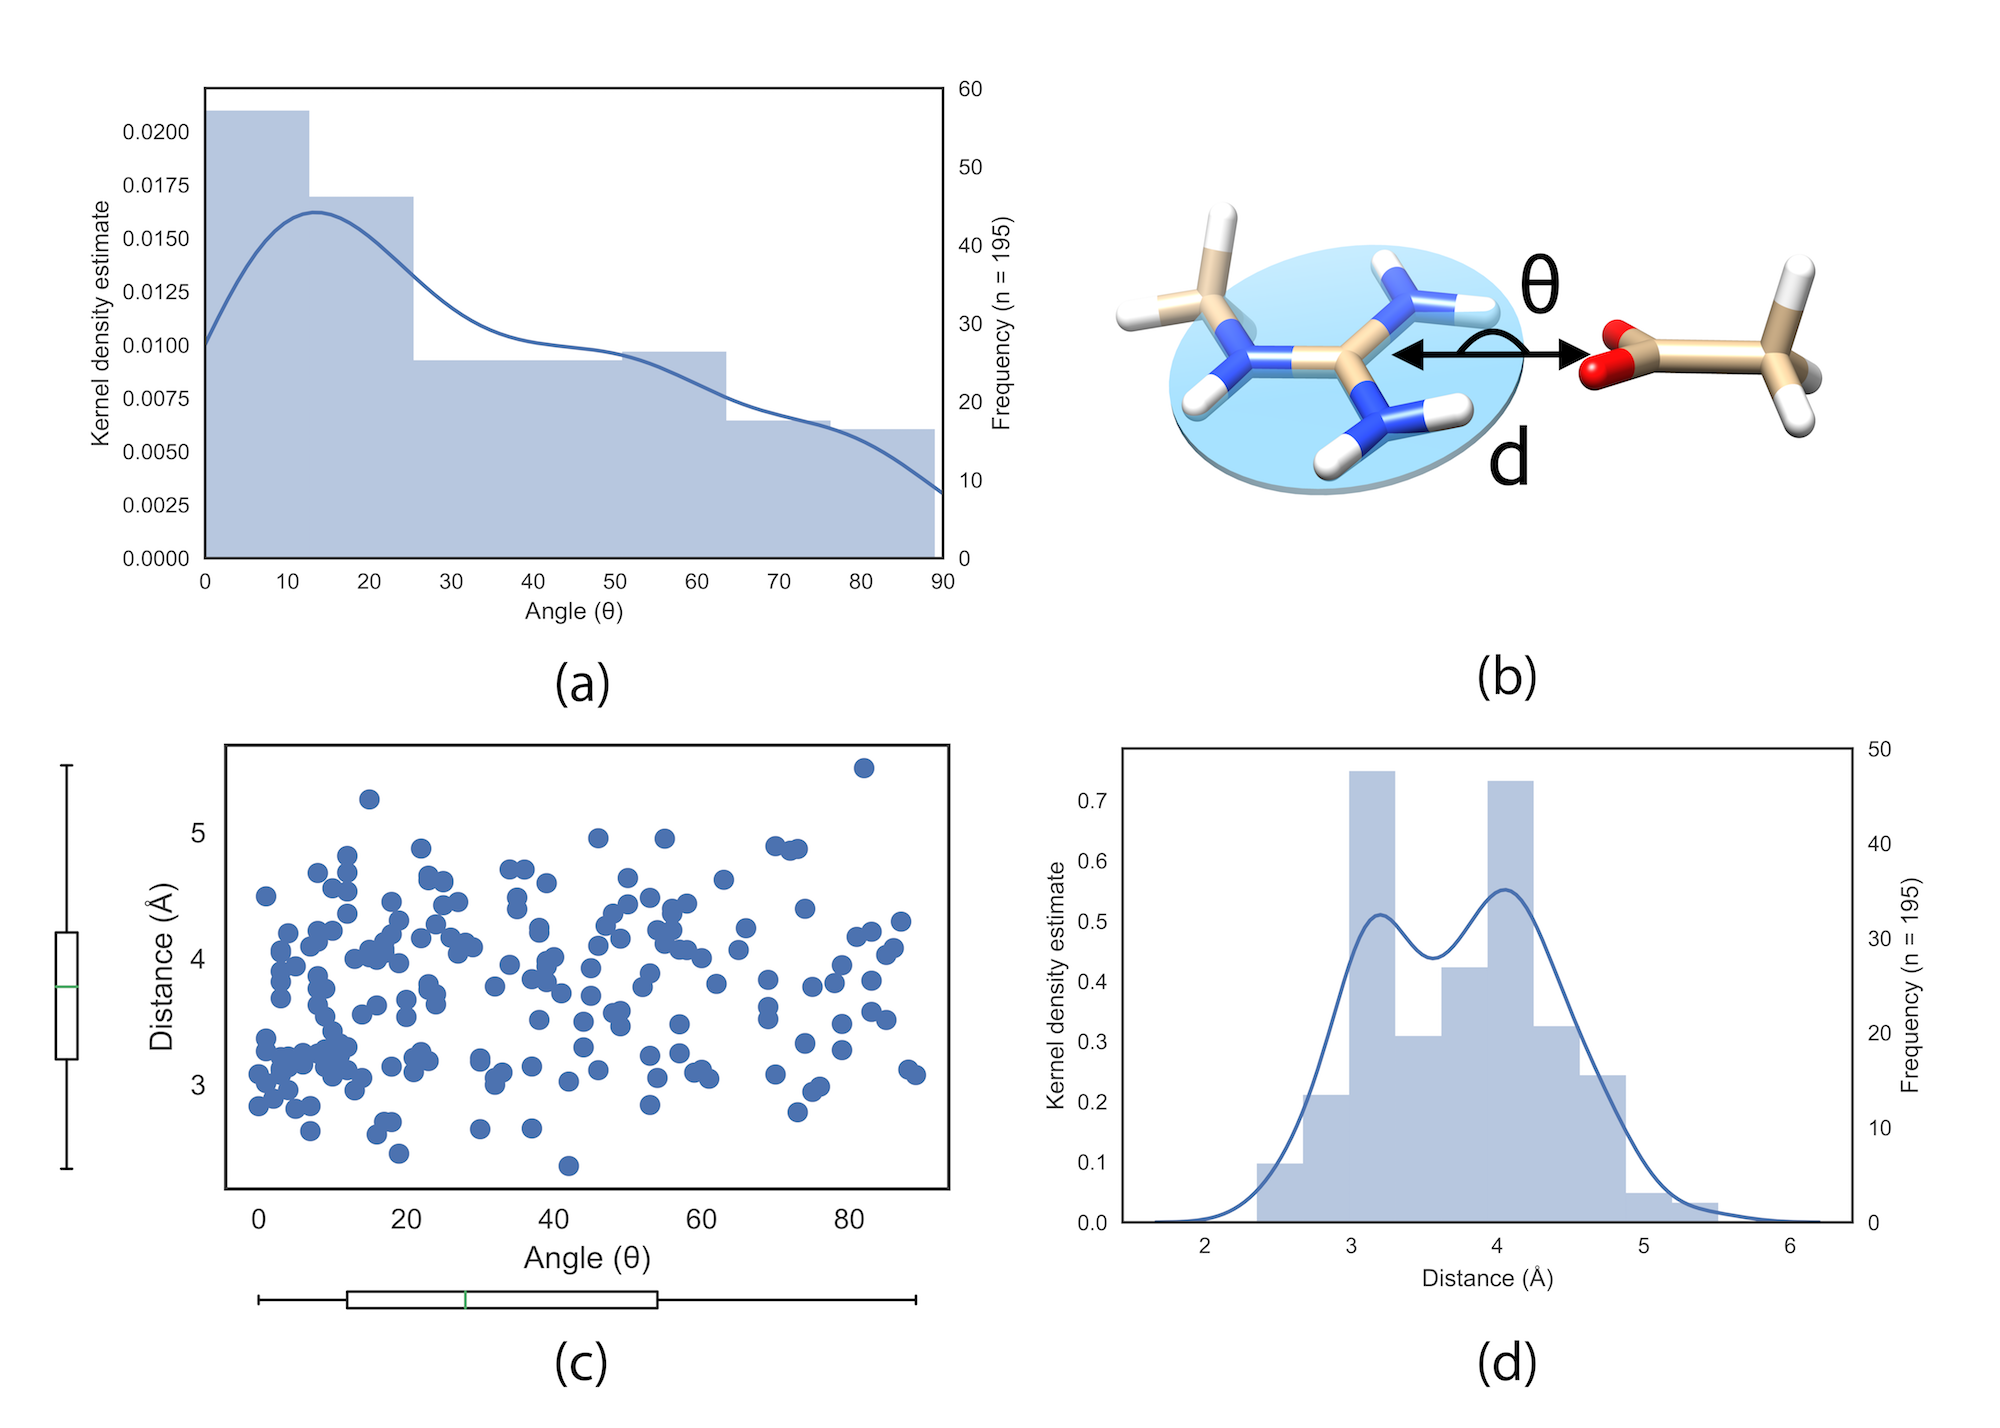
\includegraphics[width=9cm]{Figures/Datamining/arg_carb.png}
    \caption{
    % Distribution of (a) dihedral angles between arginine rings and sulfates and (d) \ce{S\bond{-}O- \bond{...}NH2+} distances shown using histogram and kernel density estimate. (b) Graphical representation of the interaction investigated. Distances and angles are shown. (c) Scatter plot of angles and distances suggests no clear relationship. The distribution of each variable is also shown using a boxplot.
    }
    \label{fig:my_label}
\end{figure}

\begin{figure}
    \centering
    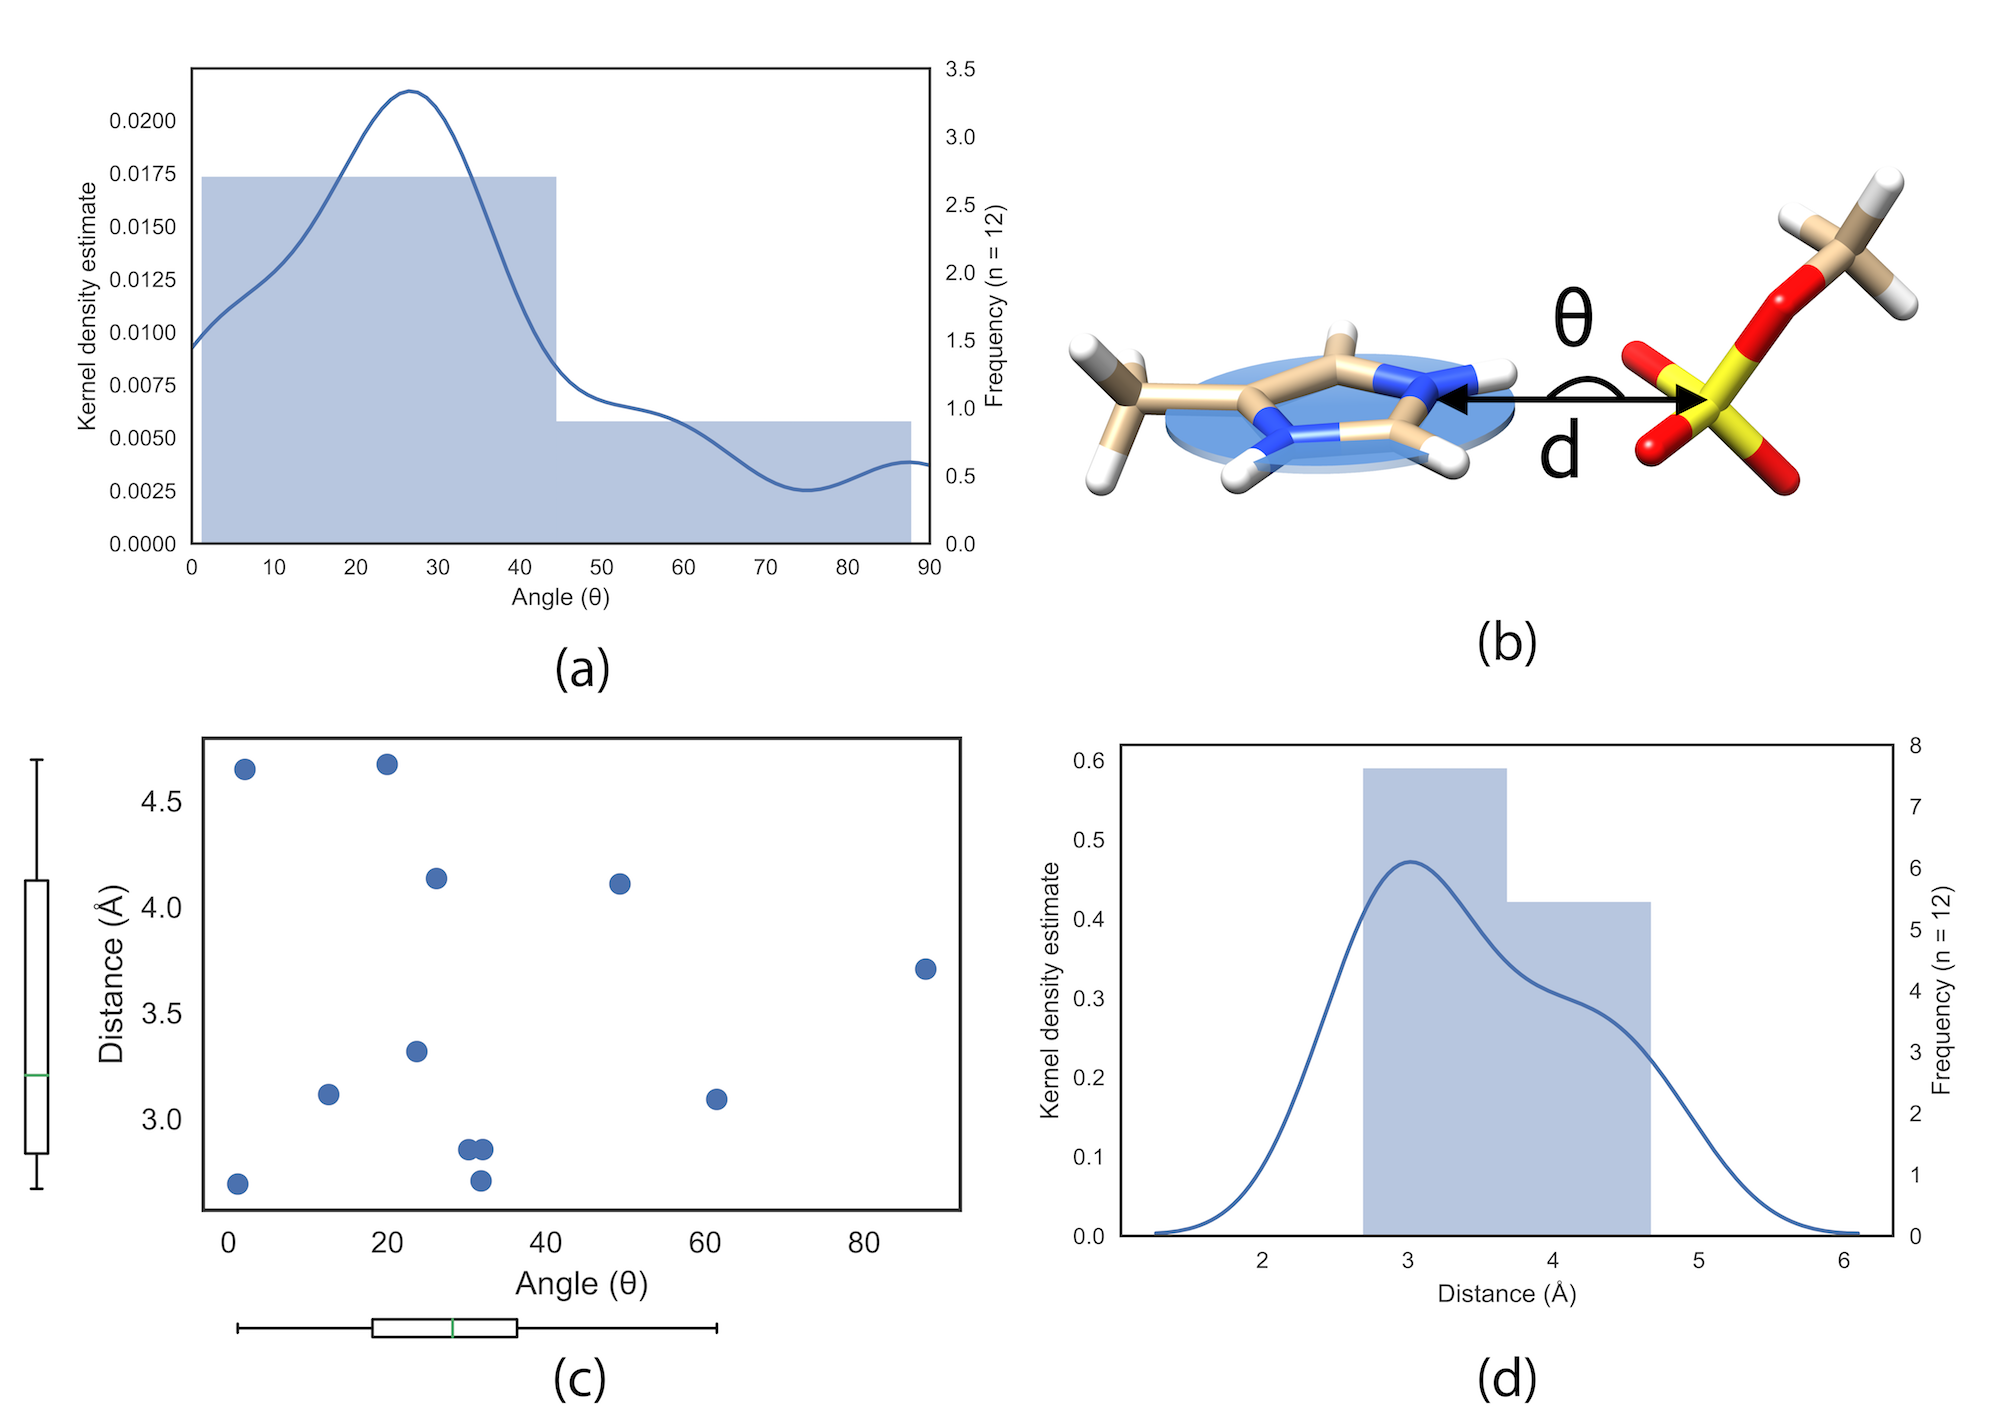
\includegraphics[width=9cm]{Figures/Datamining/hist_sulfate.png}
    \caption{
    % Distribution of (a) dihedral angles between arginine rings and sulfates and (d) \ce{S\bond{-}O- \bond{...}NH2+} distances shown using histogram and kernel density estimate. (b) Graphical representation of the interaction investigated. Distances and angles are shown. (c) Scatter plot of angles and distances suggests no clear relationship. The distribution of each variable is also shown using a boxplot.
    }
    \label{fig:my_label}
\end{figure}

\begin{figure}
    \centering
    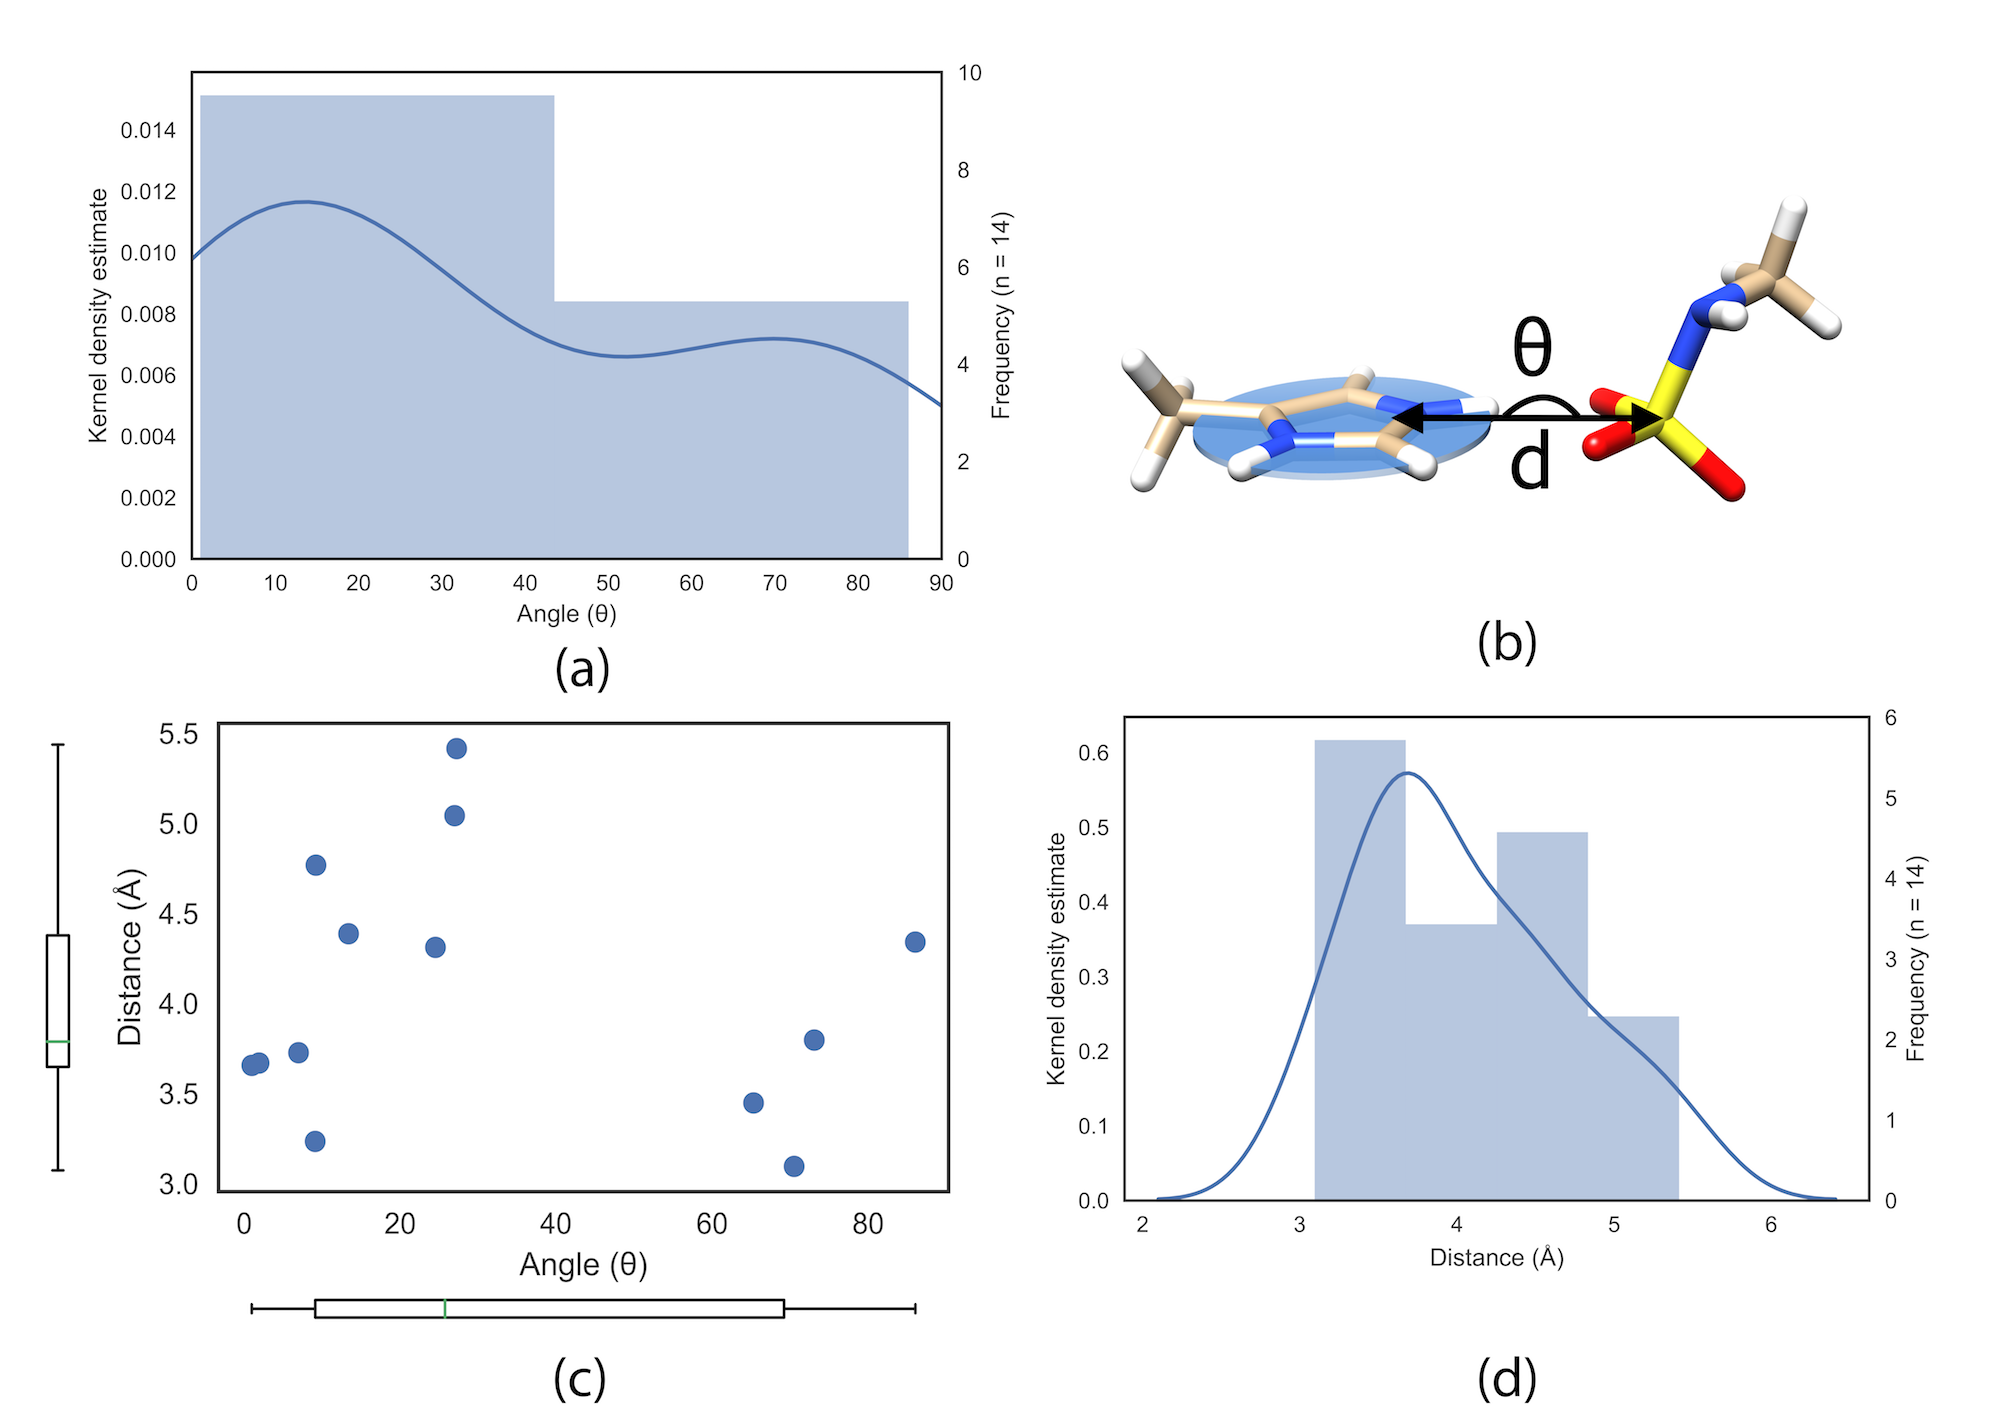
\includegraphics[width=9cm]{Figures/Datamining/his_Nsulf.png}
    \caption{
    % Distribution of (a) dihedral angles between arginine rings and sulfates and (d) \ce{S\bond{-}O- \bond{...}NH2+} distances shown using histogram and kernel density estimate. (b) Graphical representation of the interaction investigated. Distances and angles are shown. (c) Scatter plot of angles and distances suggests no clear relationship. The distribution of each variable is also shown using a boxplot.
    }
    \label{fig:my_label}
\end{figure}

\begin{figure}
    \centering
    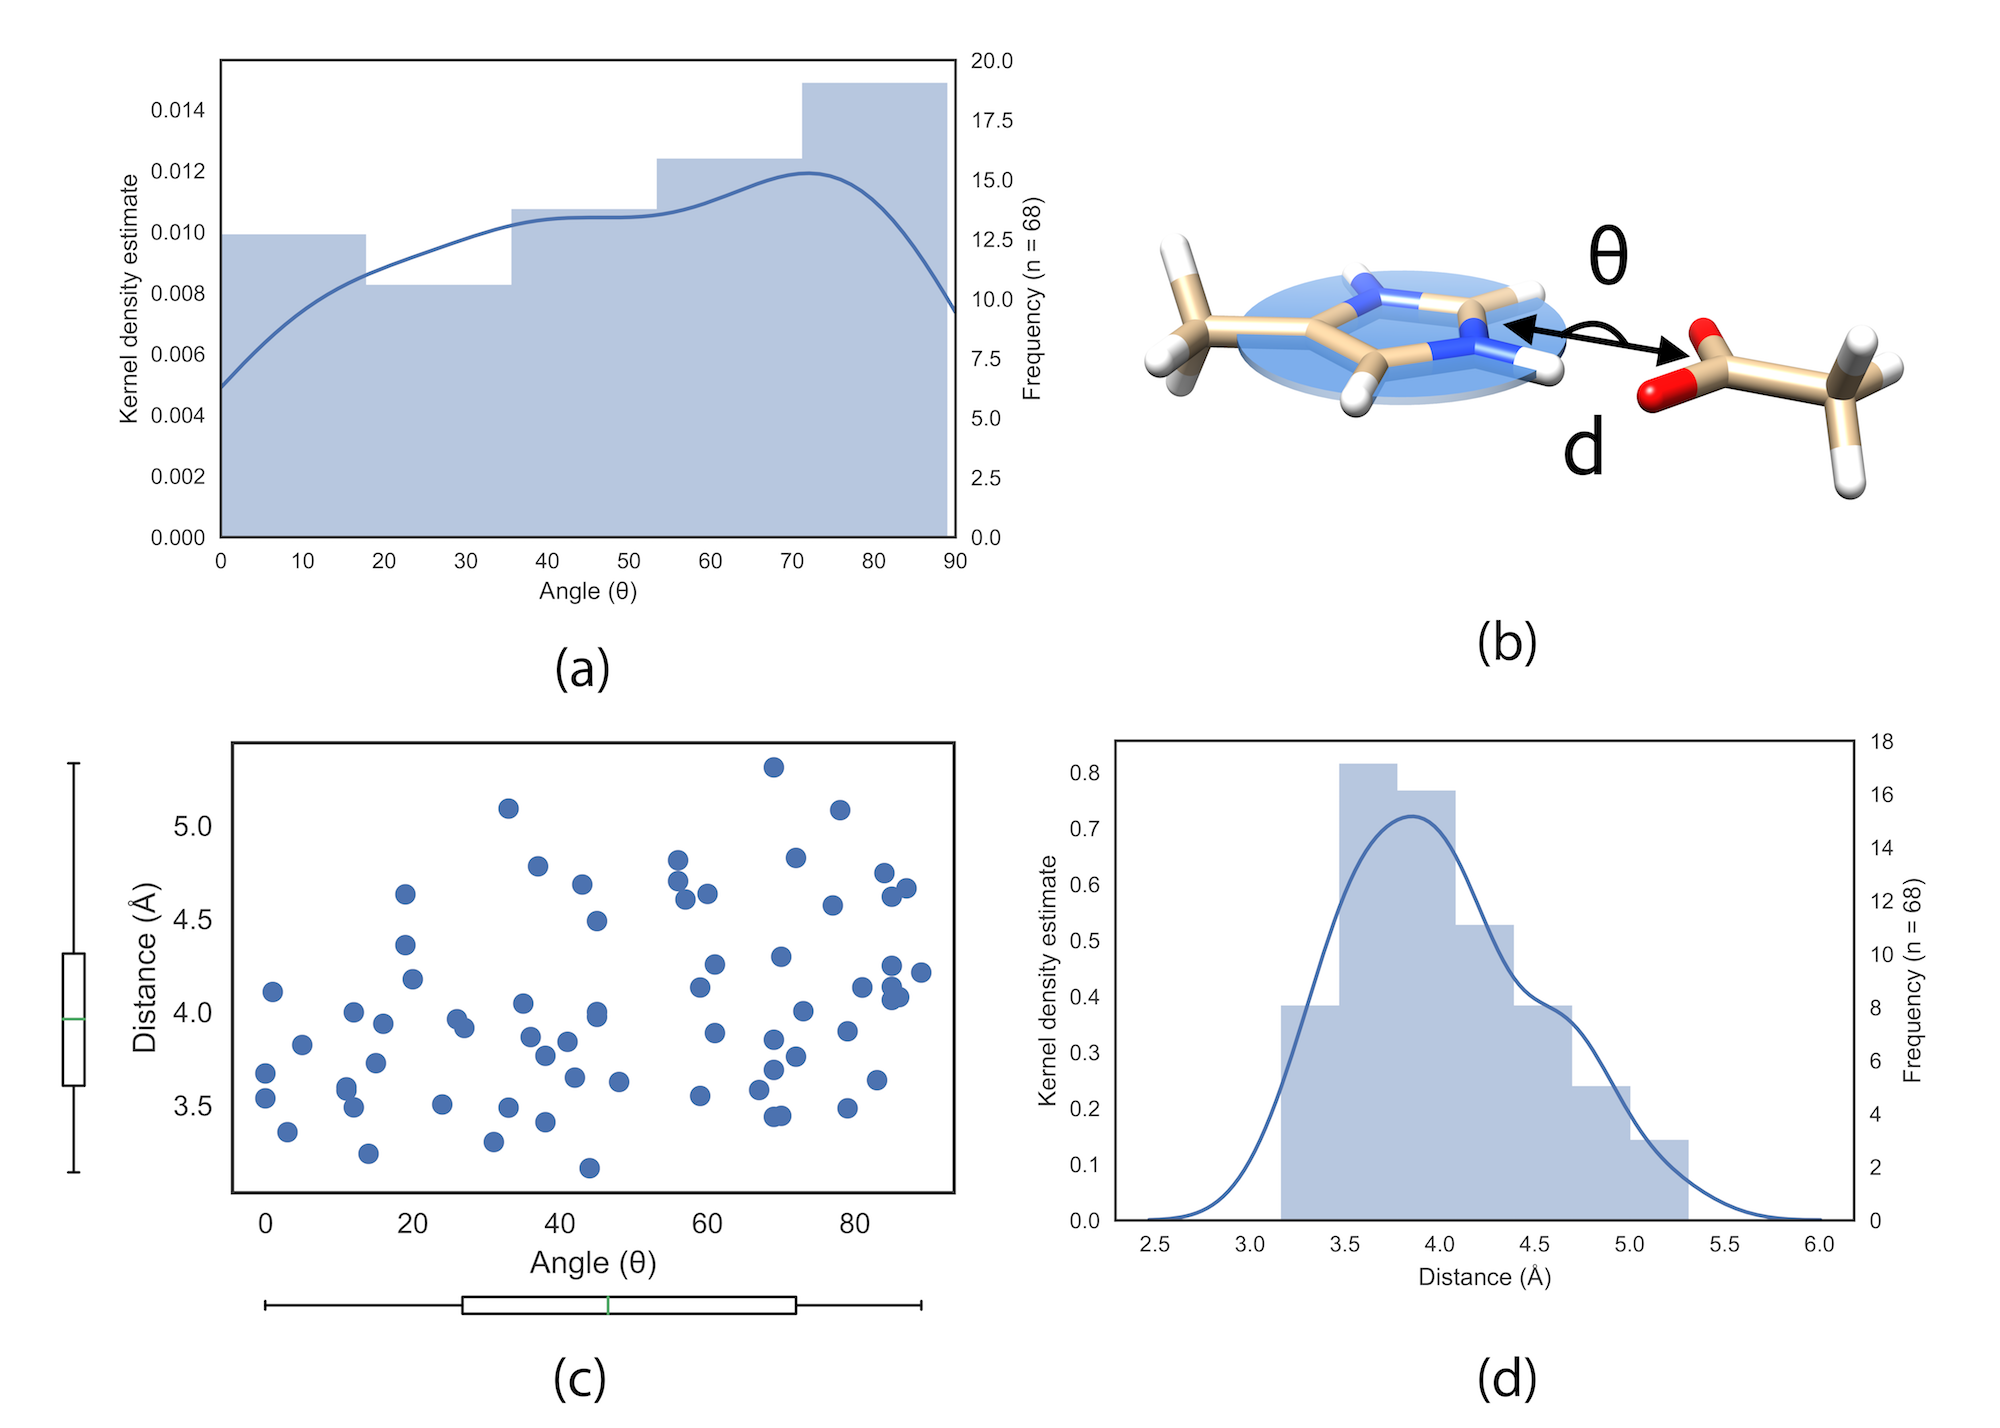
\includegraphics[width=9cm]{Figures/Datamining/his_carb.png}
    \caption{
    % Distribution of (a) dihedral angles between arginine rings and sulfates and (d) \ce{S\bond{-}O- \bond{...}NH2+} distances shown using histogram and kernel density estimate. (b) Graphical representation of the interaction investigated. Distances and angles are shown. (c) Scatter plot of angles and distances suggests no clear relationship. The distribution of each variable is also shown using a boxplot.
    }
    \label{fig:my_label}
\end{figure}

\begin{figure}
    \centering
    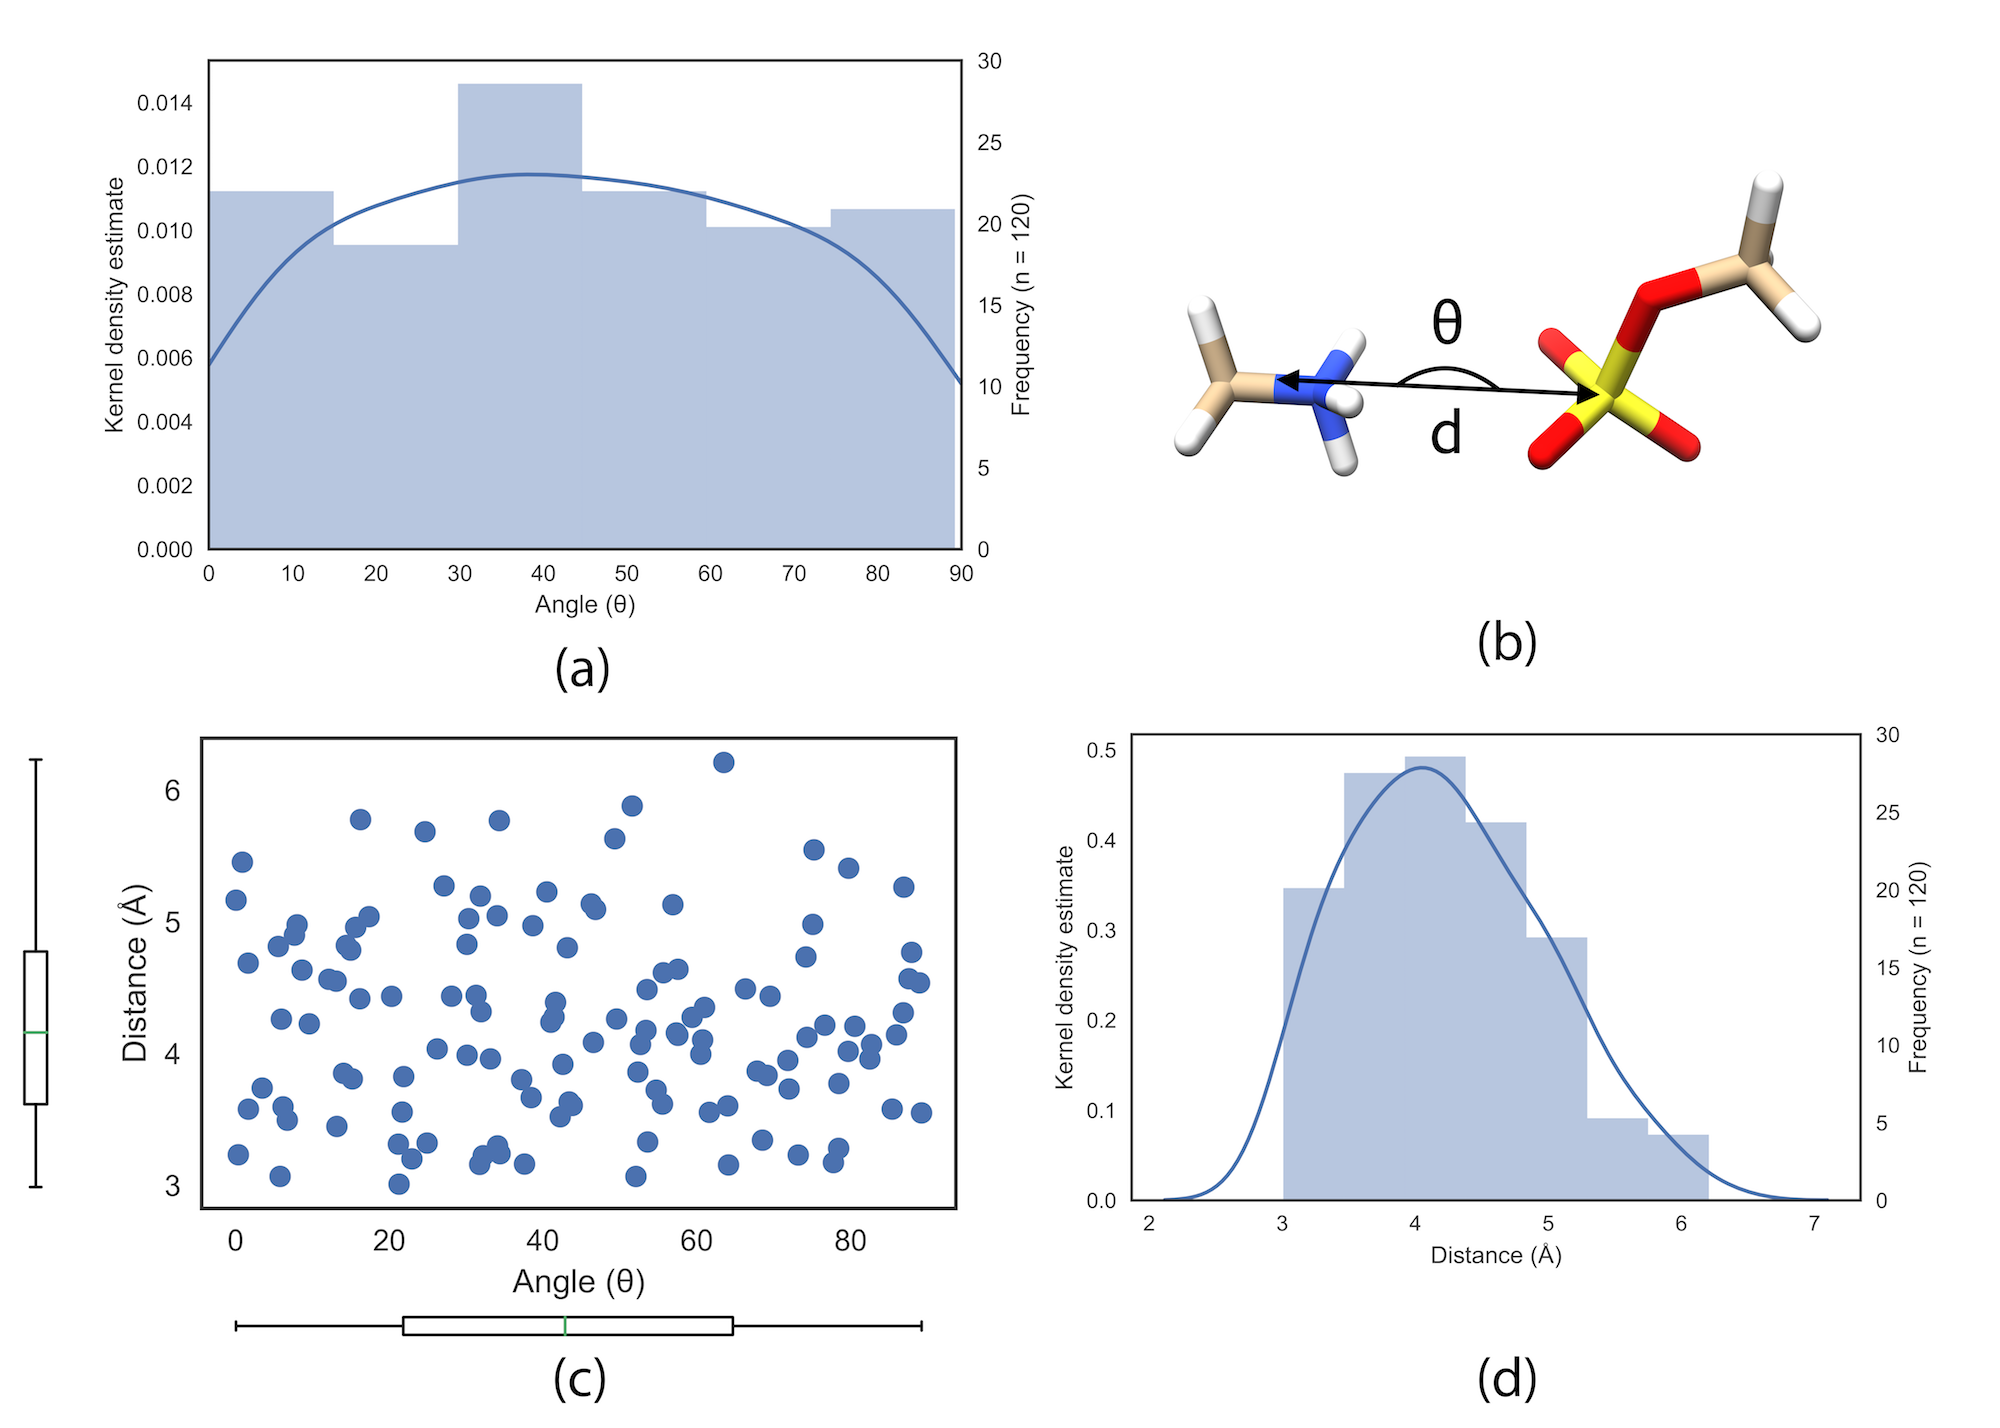
\includegraphics[width=9cm]{Figures/Datamining/lys_sulfate.png}
    \caption{
    % Distribution of (a) dihedral angles between arginine rings and sulfates and (d) \ce{S\bond{-}O- \bond{...}NH2+} distances shown using histogram and kernel density estimate. (b) Graphical representation of the interaction investigated. Distances and angles are shown. (c) Scatter plot of angles and distances suggests no clear relationship. The distribution of each variable is also shown using a boxplot.
    }
    \label{fig:my_label}
\end{figure}

\begin{figure}
    \centering
    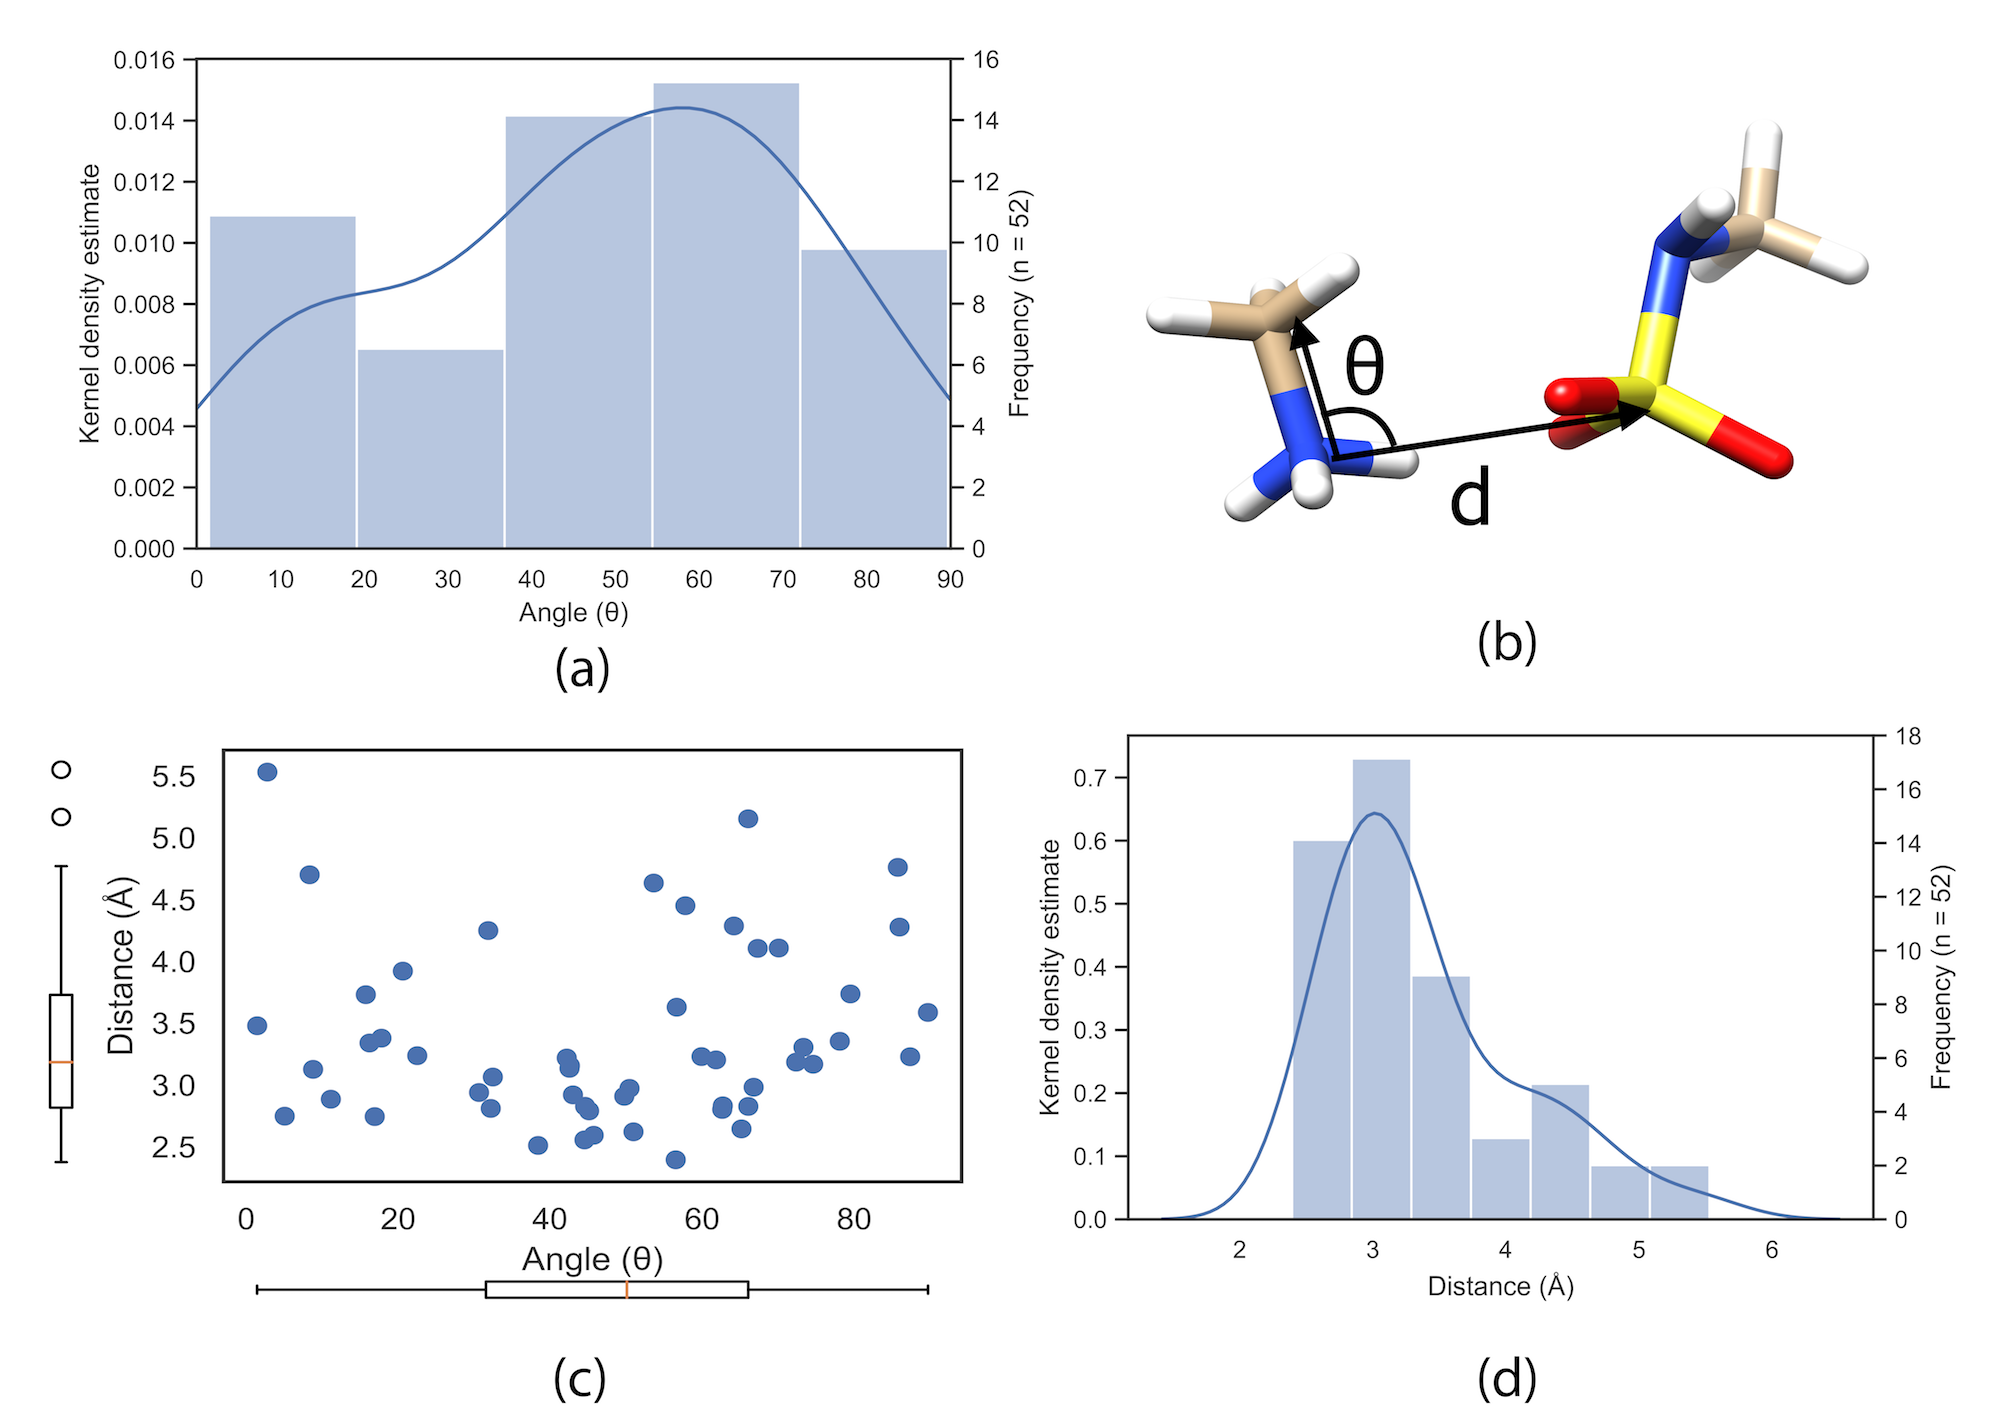
\includegraphics[width=9cm]{Figures/Datamining/lys_Nsulfate.png}
    \caption{
    % Distribution of (a) dihedral angles between arginine rings and sulfates and (d) \ce{S\bond{-}O- \bond{...}NH2+} distances shown using histogram and kernel density estimate. (b) Graphical representation of the interaction investigated. Distances and angles are shown. (c) Scatter plot of angles and distances suggests no clear relationship. The distribution of each variable is also shown using a boxplot.
    }
    \label{fig:my_label}
\end{figure}

\begin{figure}
    \centering
    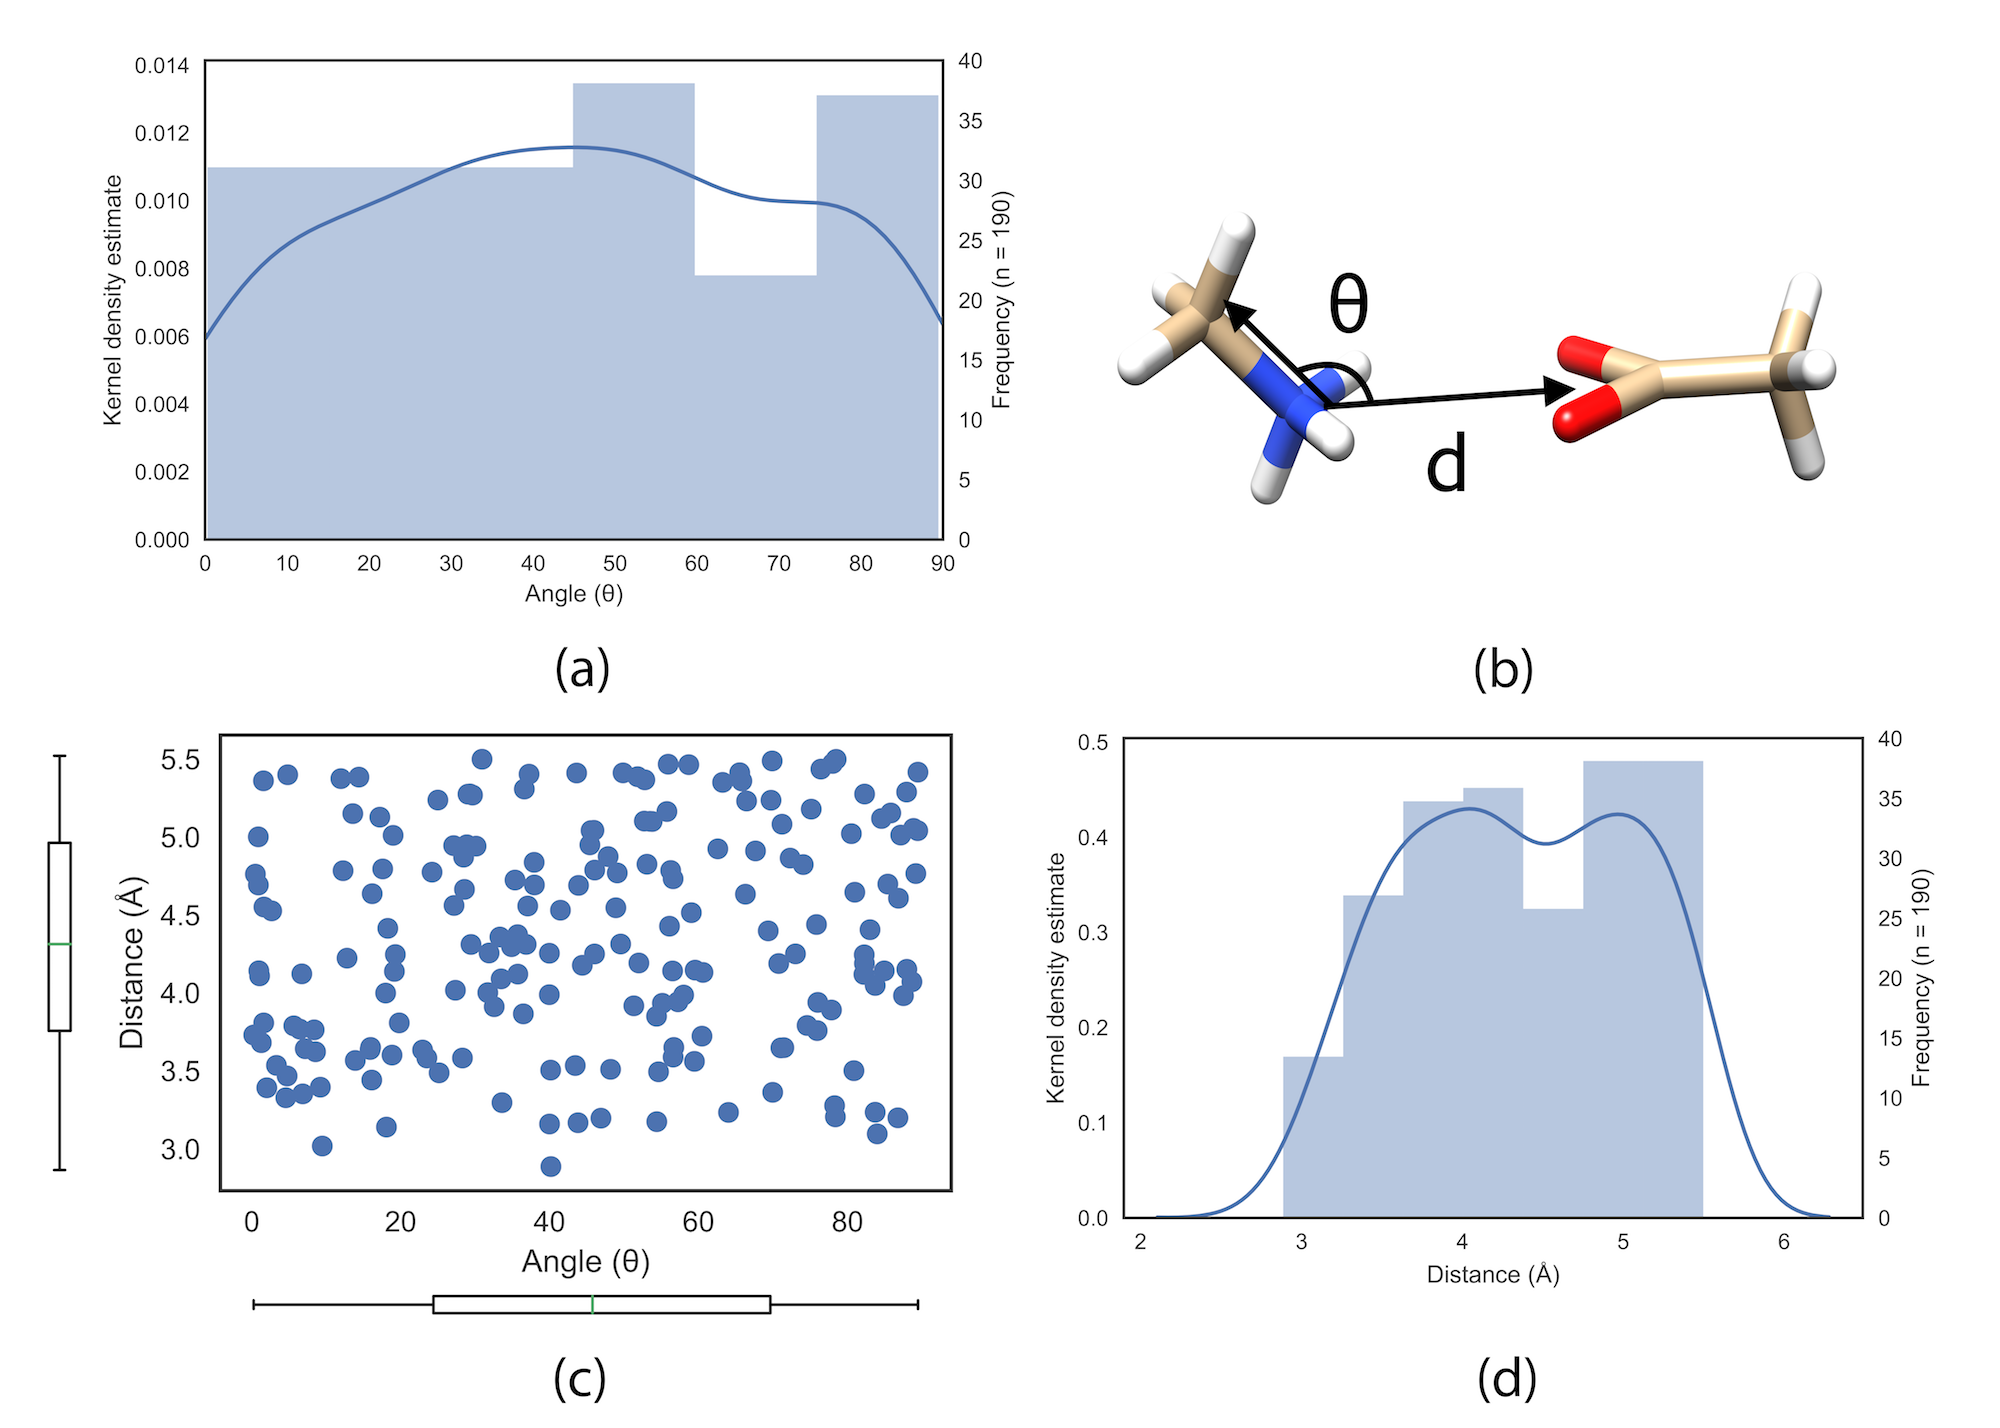
\includegraphics[width=9cm]{Figures/Datamining/lys_carb.png}
    \caption{
    % Distribution of (a) dihedral angles between arginine rings and sulfates and (d) \ce{S\bond{-}O- \bond{...}NH2+} distances shown using histogram and kernel density estimate. (b) Graphical representation of the interaction investigated. Distances and angles are shown. (c) Scatter plot of angles and distances suggests no clear relationship. The distribution of each variable is also shown using a boxplot.
    }
    \label{fig:my_label}
\end{figure}


\section{Results and Discussion}



\chapter{Development of a Glycosaminoglycan Specific Scoring Function}

\section{Glycosidic Torsion Energy Penalty Functions}
\subsection{Methods}
\noindent \textbf{Preparing the Model Structures}\\
Glycosidic linkages between disaccharides were modelled using two molecules of tetrahydropyran (THP). THP has been used extensively as a minimal model system for investigating the rotational parameters of the glycosidic torsion. Two reasons for this practice are commonly cited: (1) it less computationally expensive than using the entire disaccharide structure (THP only requires a fraction of the basis functions for QM calculations compared to the full structure) and (2) it disambiguates other interaction energies (e.g. intramolecular hydrogen bonds between hydroxyl groups) from the energy reported. In regards to the latter, it is argued that, even without the confounding energies from intramolecular hydrogen bonding, the electronic free energy of the glycosidic torsion is undoubtedly dependent on the substituents of the ring and their orientation in space. However, while this model may be an  oversimplification, its predictive power to locate ranges of low energy glycosidic torsions has been demonstrated.\autocite{Nivedha2015}  

Starting ring conformations and linkages of the THP molecules were taken from exemplary geometries from crystal structures in the PDB. All other substituents were removed and replaced with hydrogens. 

\noindent \textbf{Quantum Mechanics Calculations}\\
These structures were minimized at the HF/6-31+G(d) level of theory. The dihedrals \textphi~and \textpsi~were scanned using Gaussian 16's \textit{opt=ModRedundant} keyword, in increments of 15\degree~over 24 steps. Frequency and optimization calculations on each of the minimized structures across the scans was performed at the M062X functional and 6-311++G(2d,2p) basis set. The SCRF solvent model for water was also included. During optimization, the glycosidic torsional angle was kept fixed, which allowed for a relaxed potential energy scan. 

\noindent \textbf{Fitting the Model}\\
For each glyocosidic torsional energy profile, a series of Gaussian curves (equation \ref{eq:2}) were used to model the data,  where $x$ is the glycosidic torsion and $a_{i}$, $b_{i}$, and $c_{i}$ correspond to the magnitude, width, and mid-point of each individual Gaussian distribution, respectively.
\begin{equation} \label{eq:2}
\begin{multlined}
$$f(x)=\sum^{N}_{i=1}a_{i}e^{-\frac{(x-b_{i})^{2}}{c_{i}}} \quad \quad 0 \leq x < 360$$
\end{multlined}
\end{equation}
\noindent This function was fit to the data using a least squares optimization, available in the Scipy library in the Python programming language, with use of the Levenberg-Marquardt Algorithm. 


\subsection{Results and Discussion}
\begin{figure}[h]
    \centering
    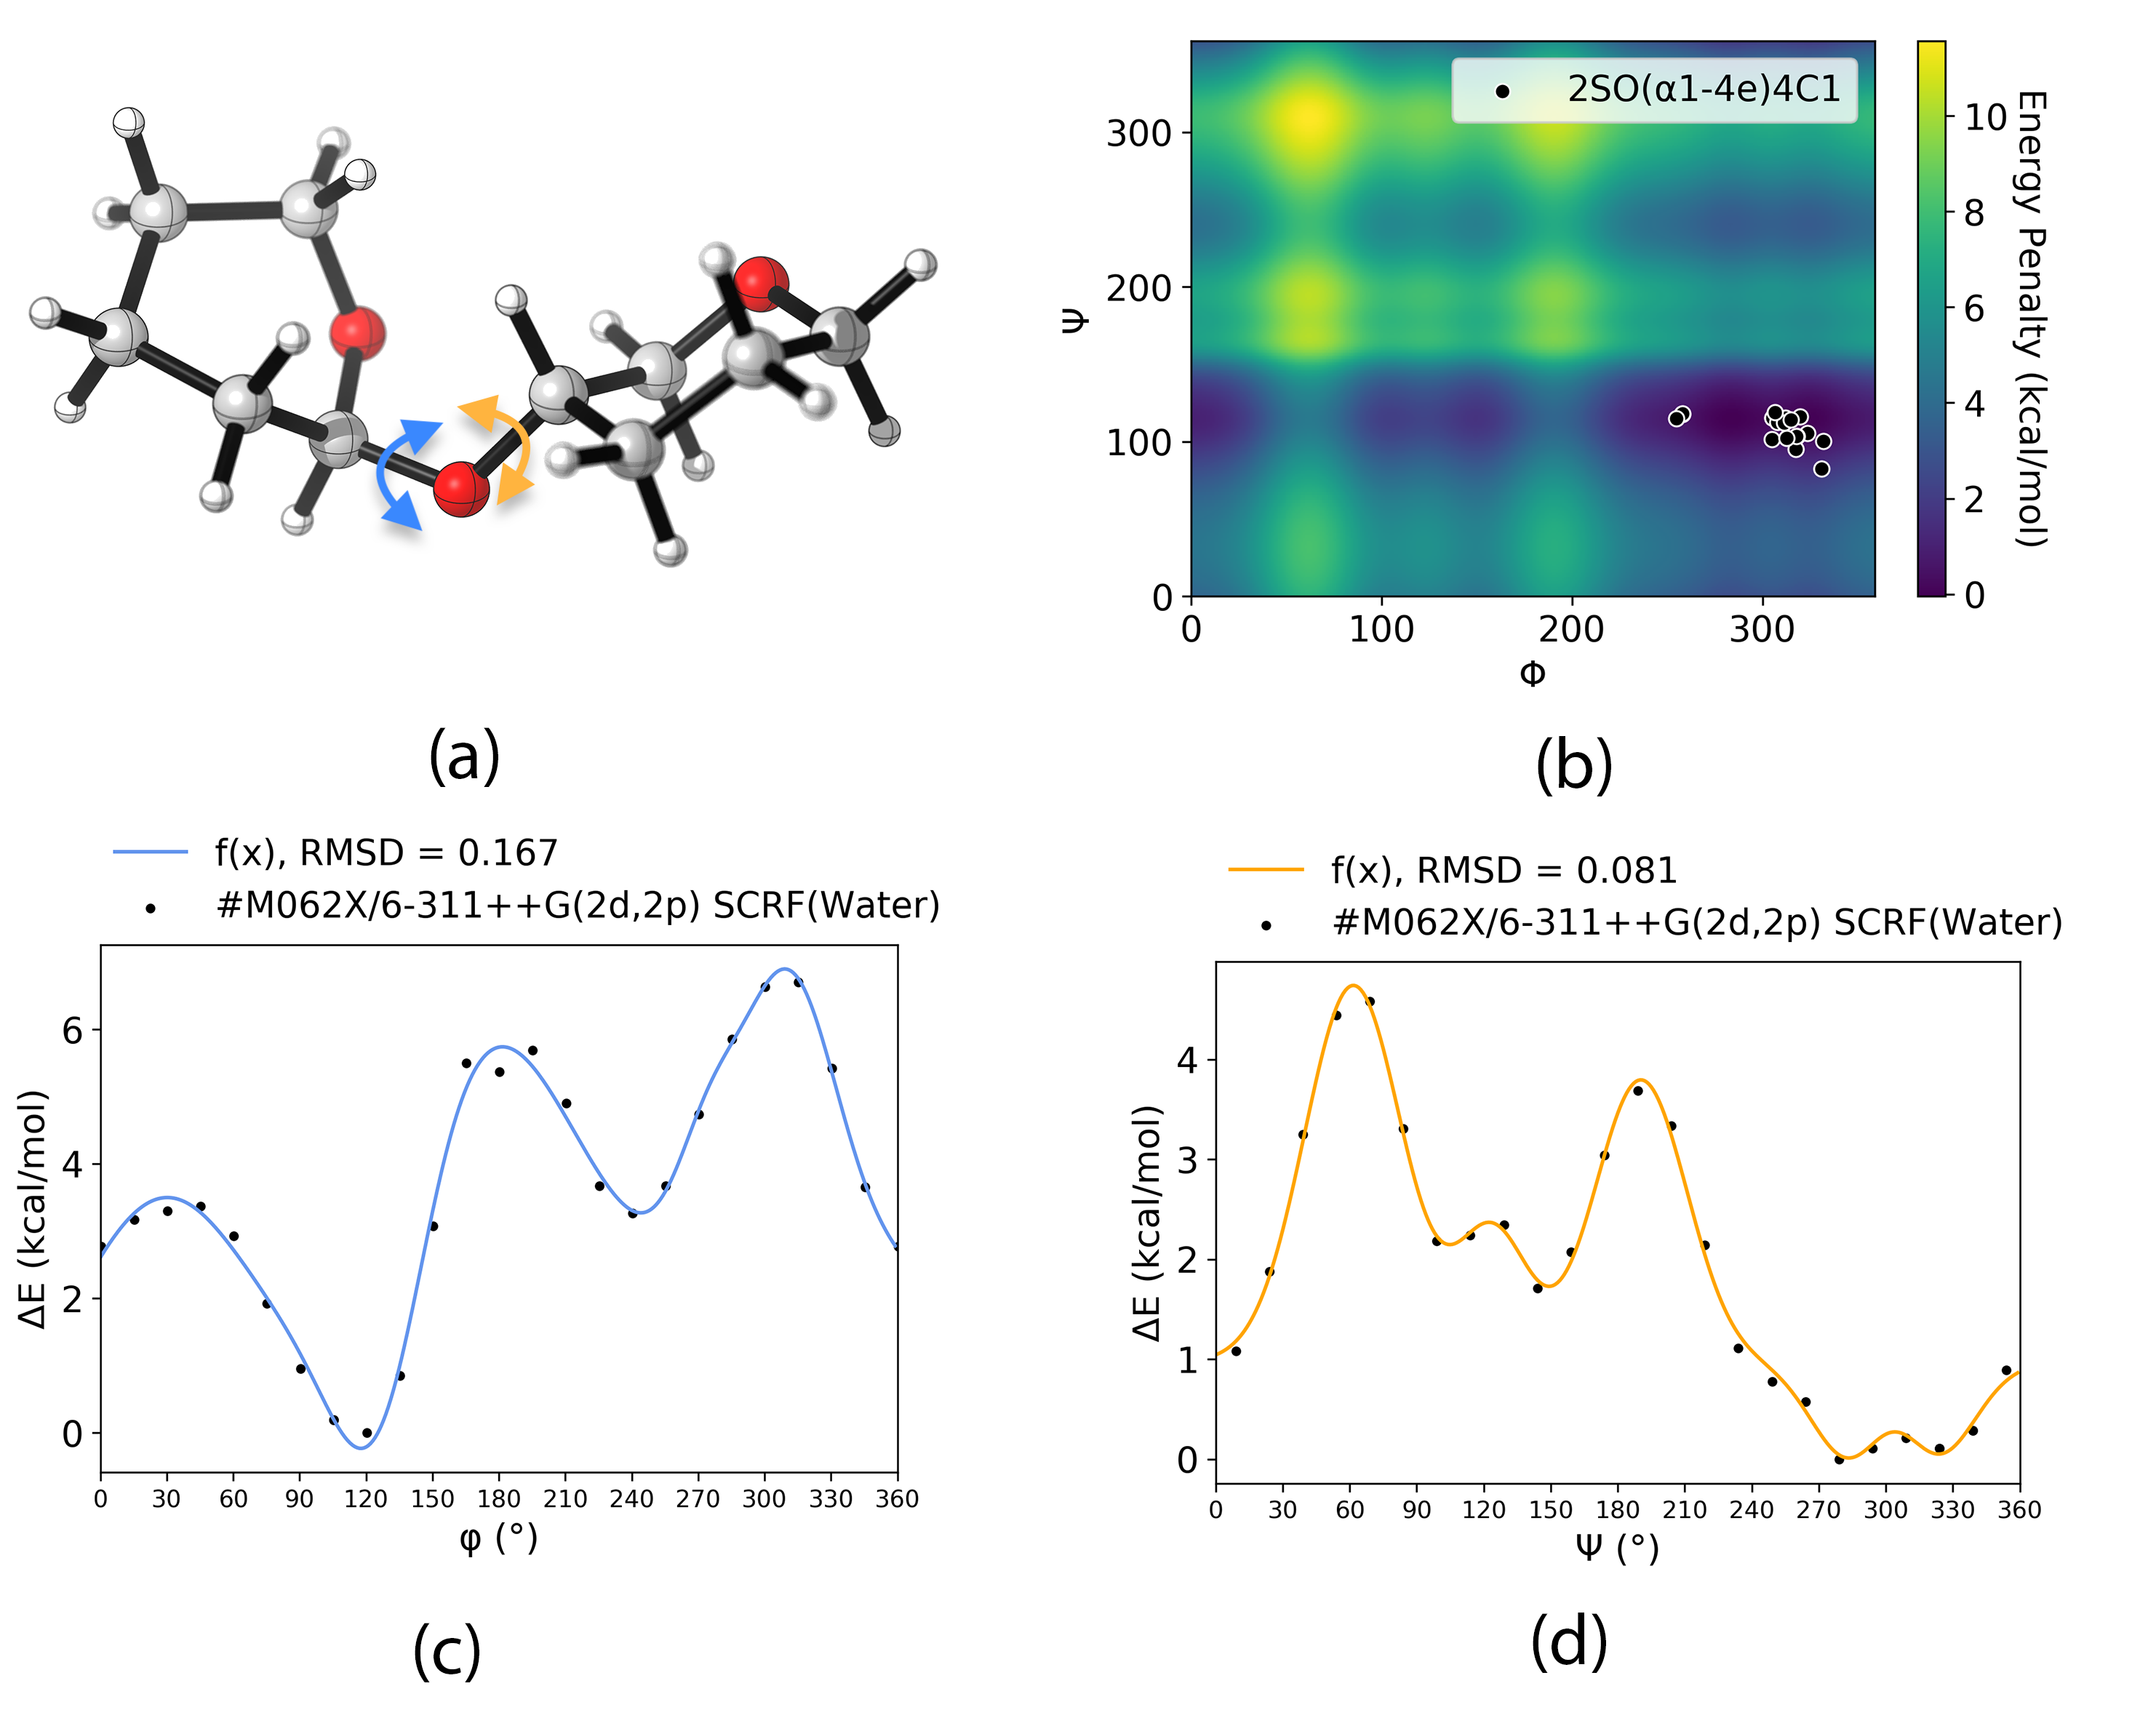
\includegraphics[width=14cm]{Figures/Torsions/2so_1c4.png}
    \caption{}
    \label{fig:2sO_4c1}
\end{figure}

\begin{figure}[h]
    \centering
    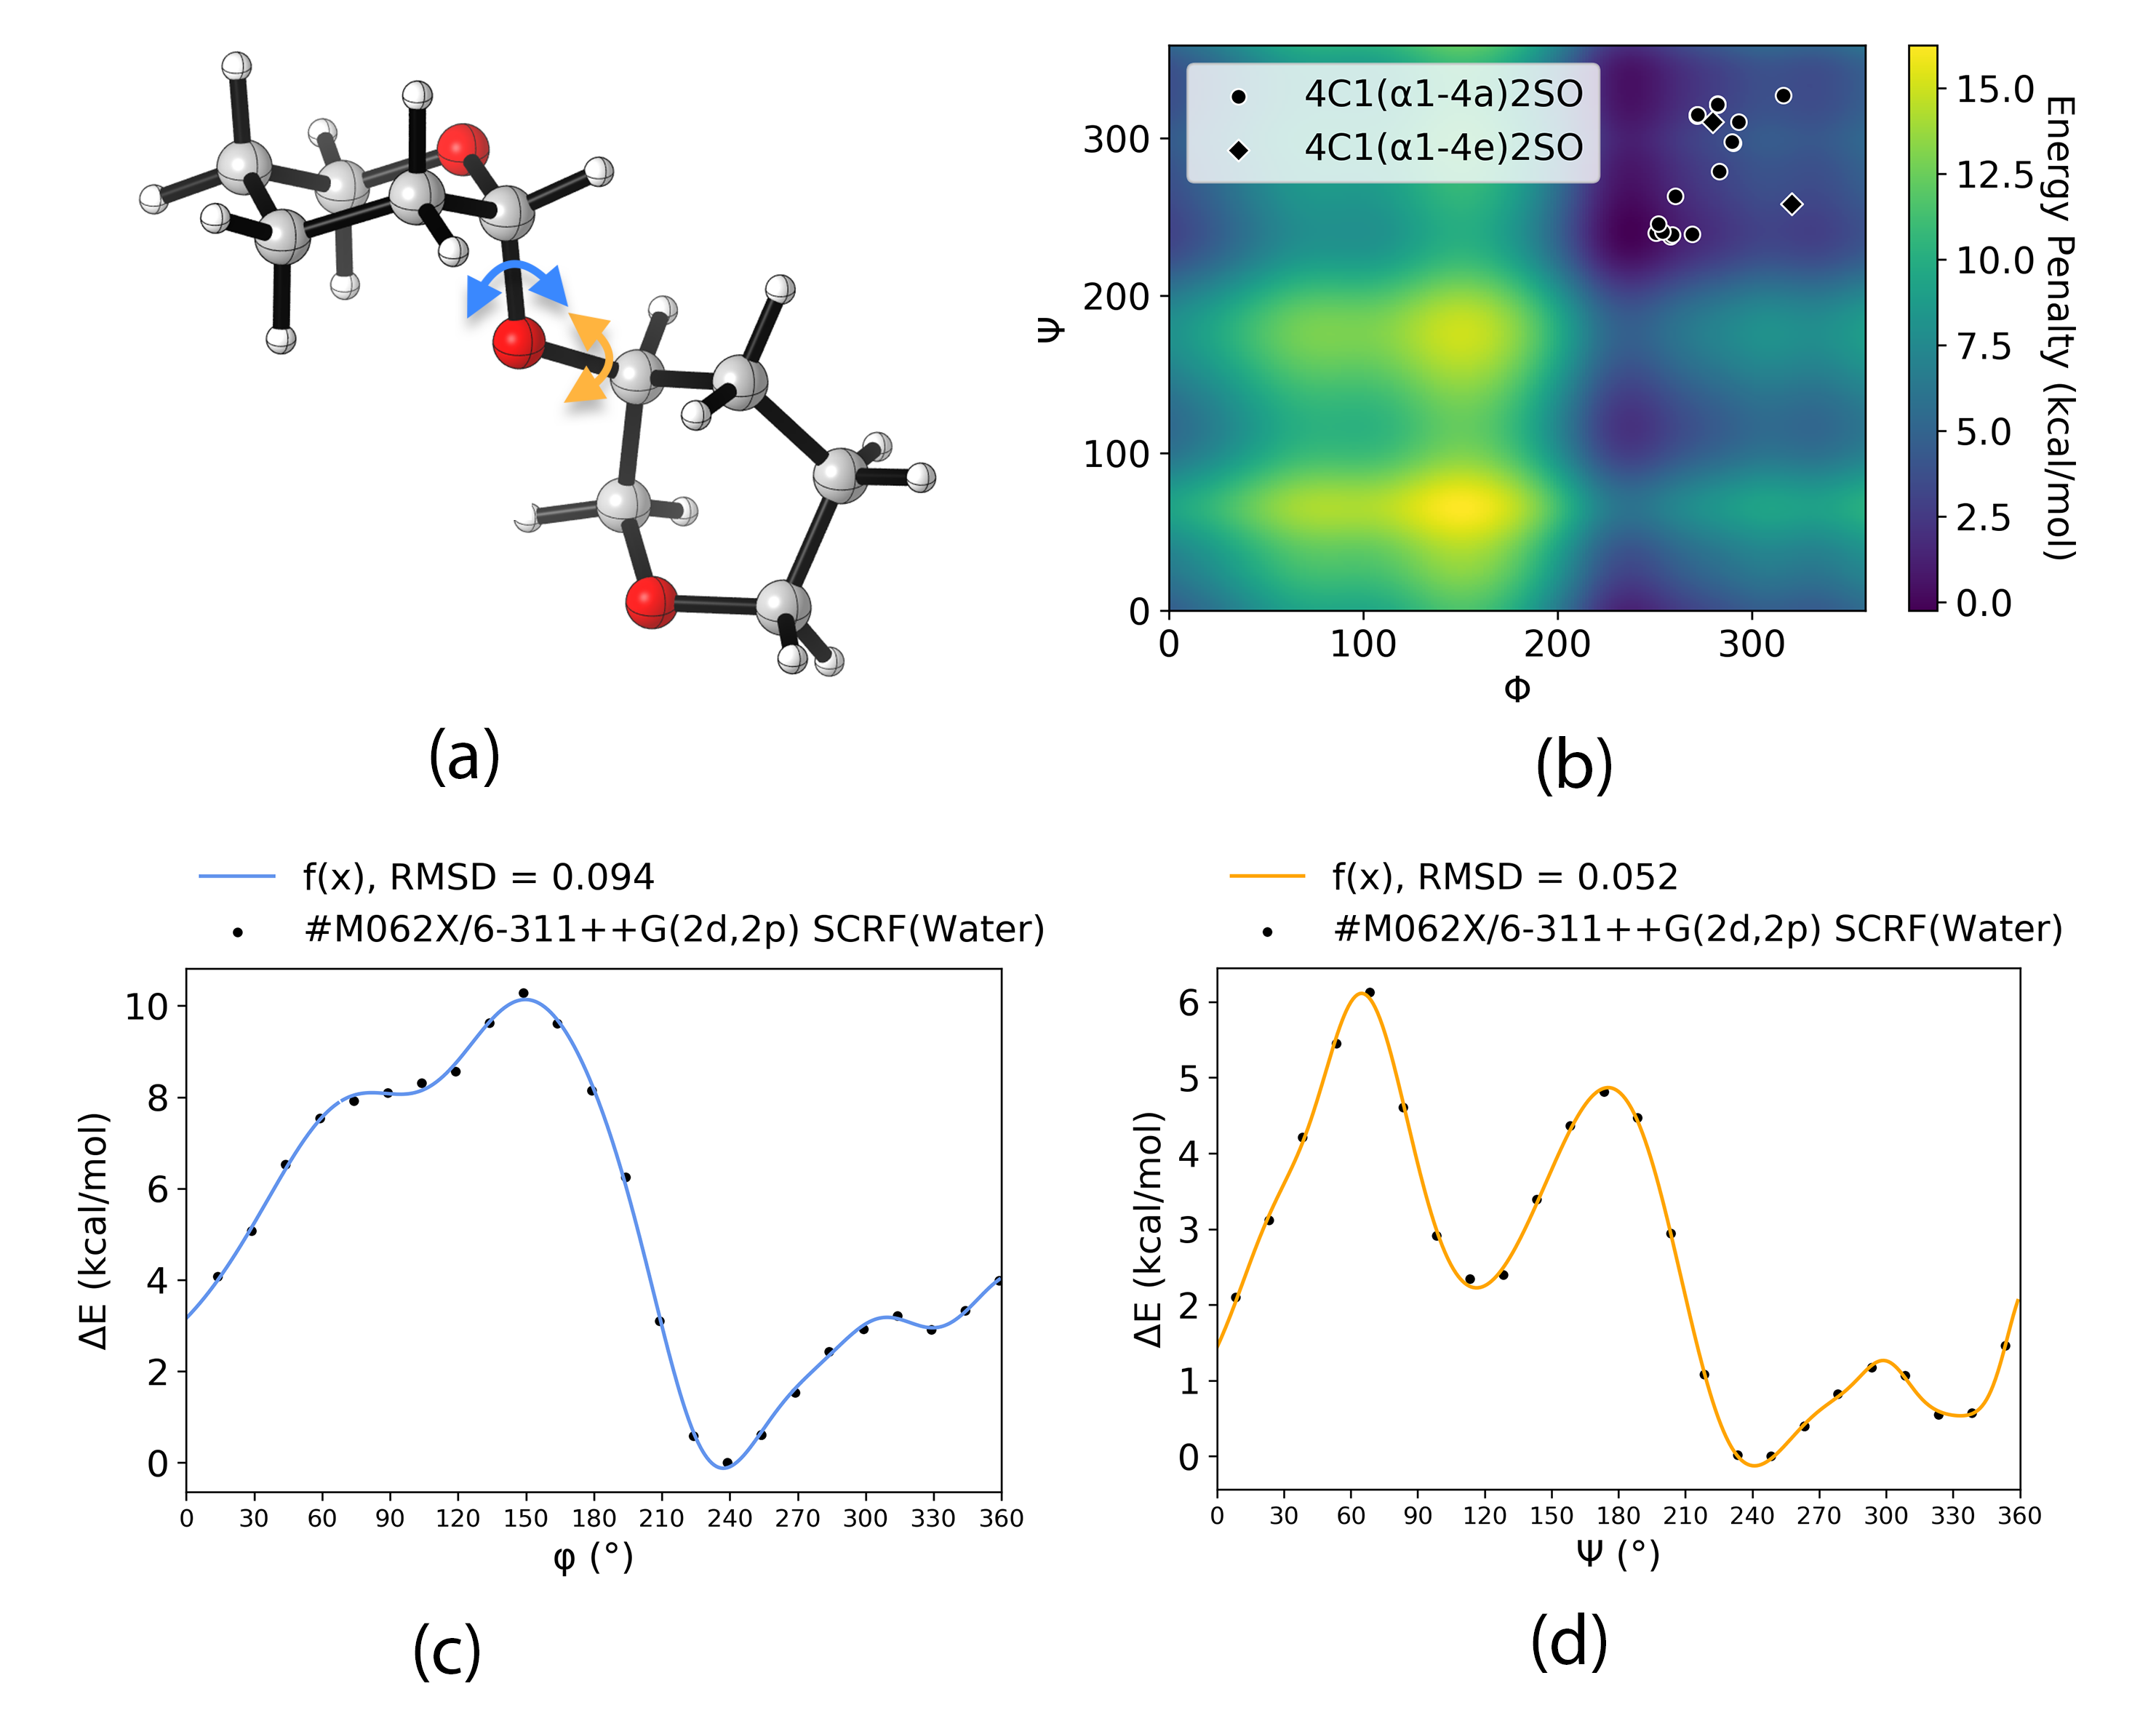
\includegraphics[width=14cm]{Figures/Torsions/4c1_a_2so.png}
    \caption{}
    \label{fig:4c1_2sO}
\end{figure}

\begin{figure}[h]
    \centering
    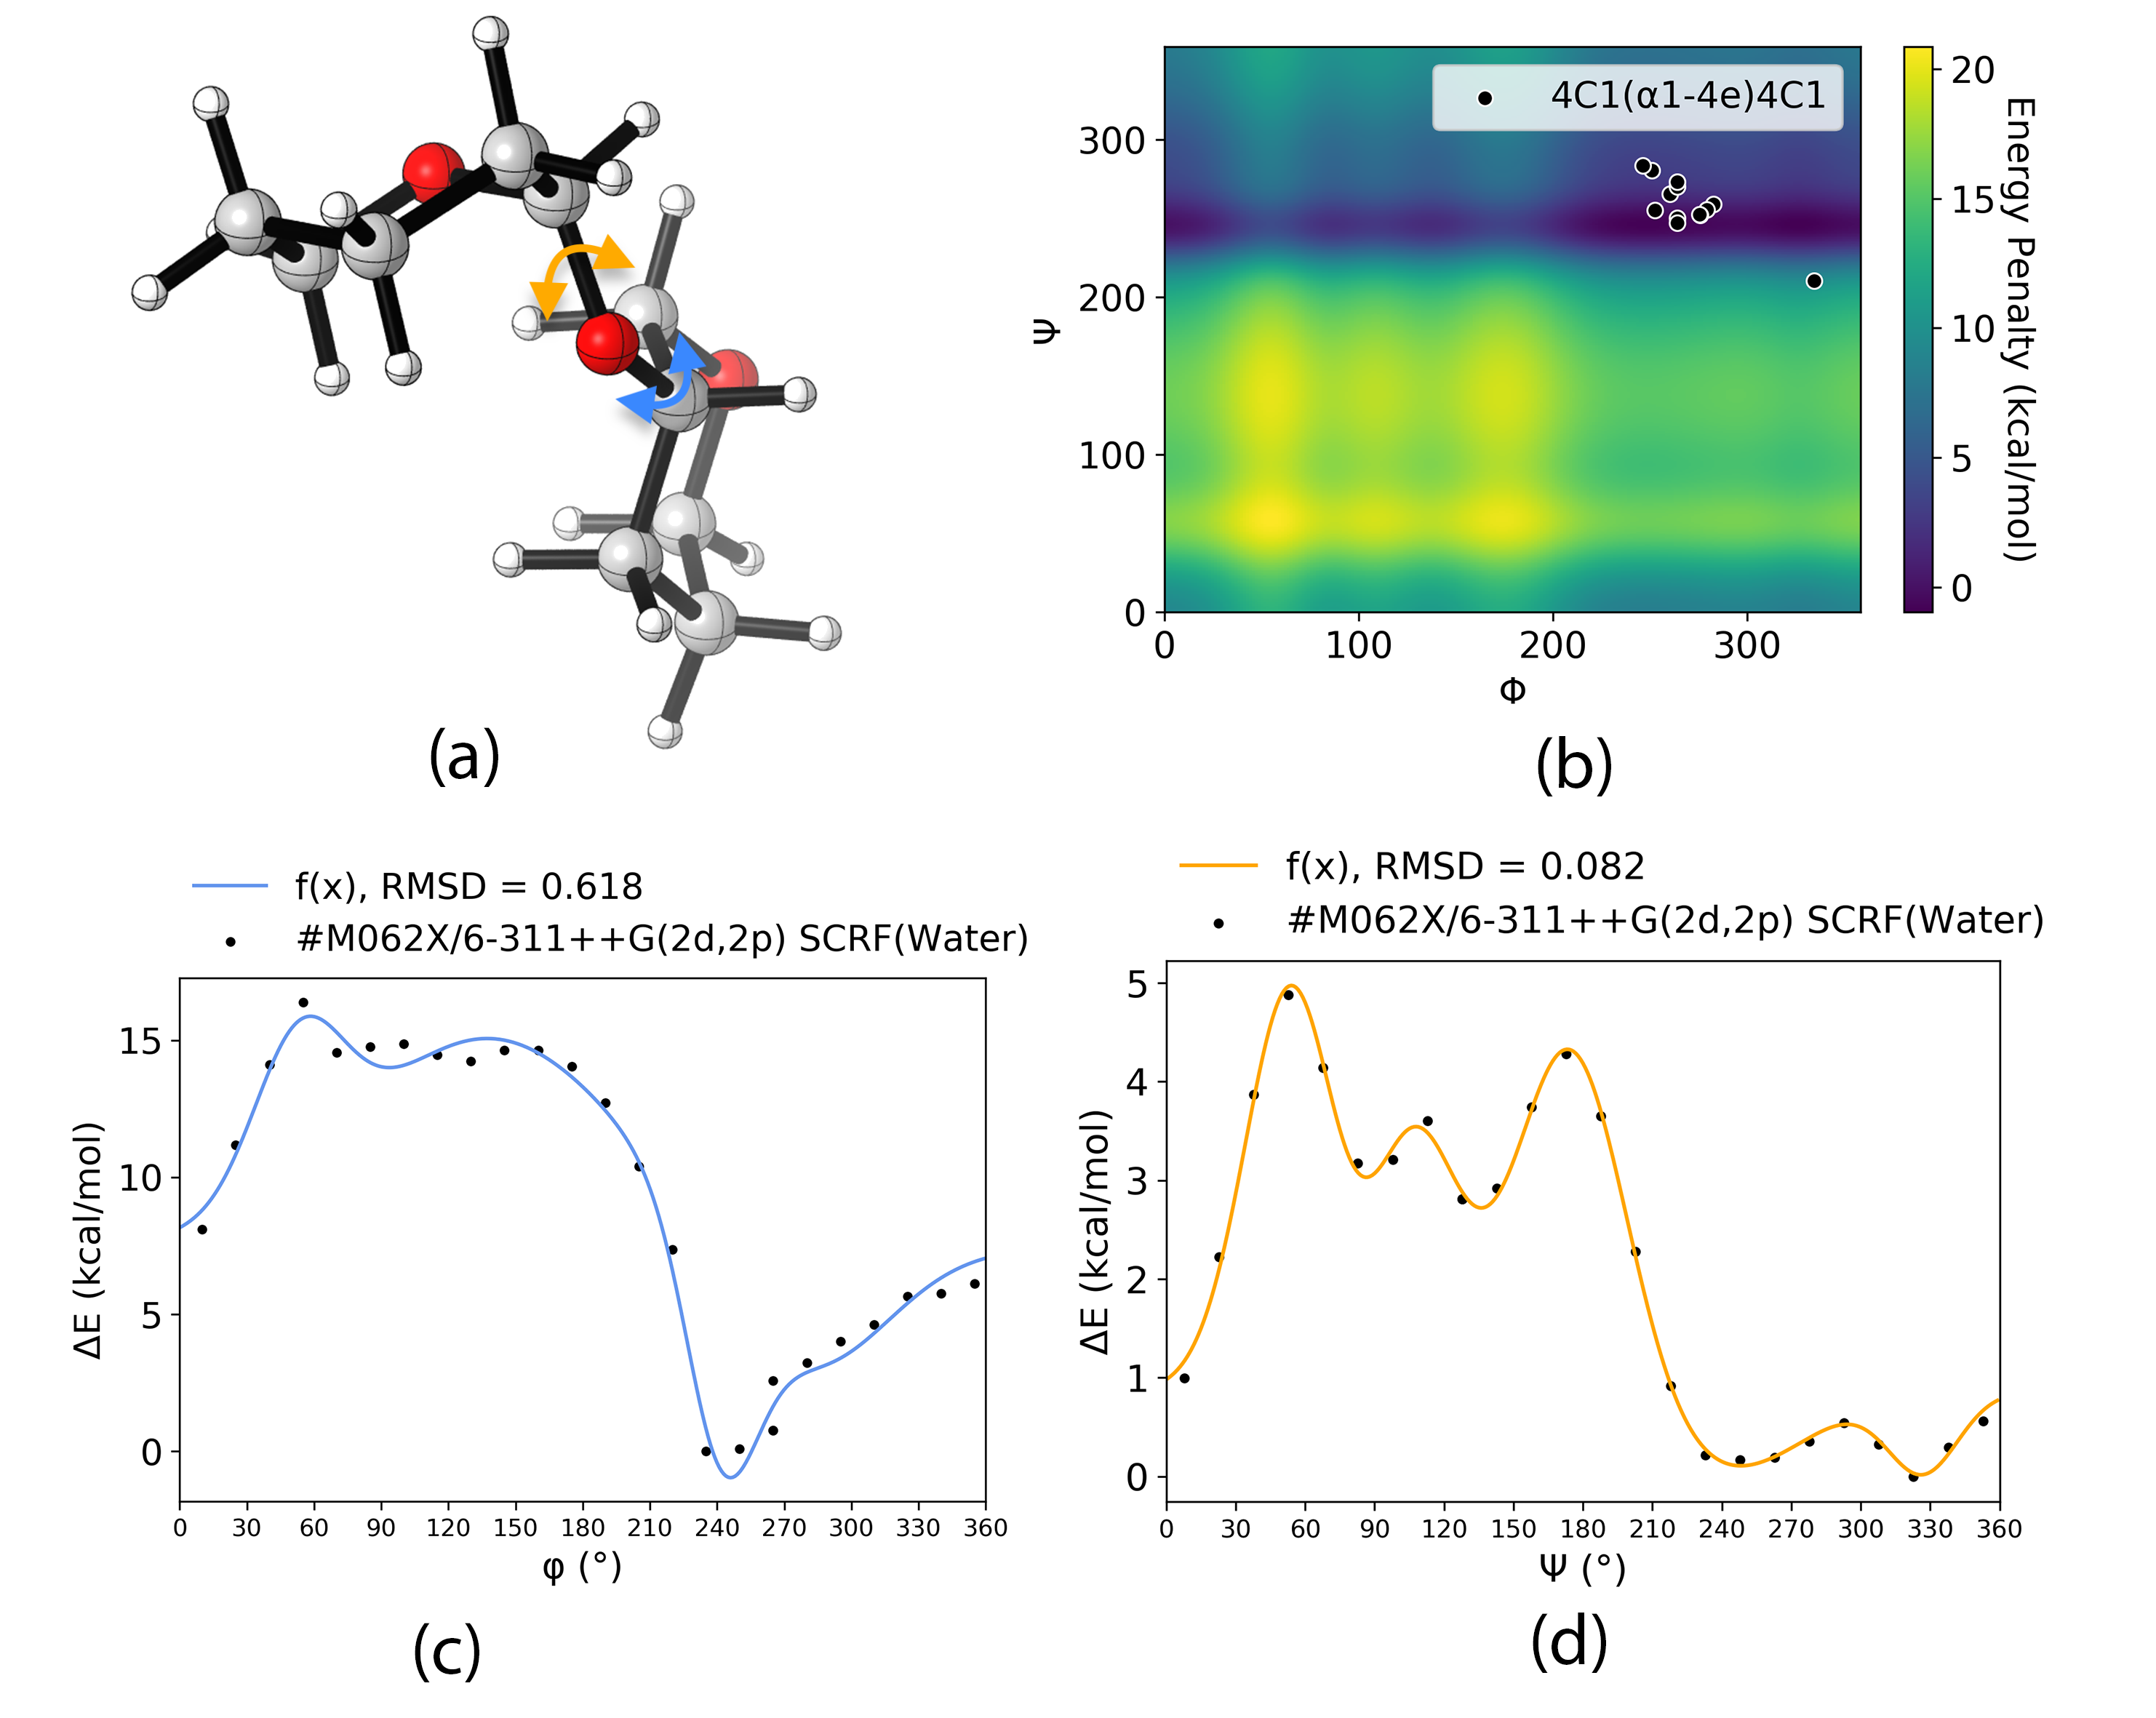
\includegraphics[width=14cm]{Figures/Torsions/Da1_4eD.png}
    \caption{}
    \label{fig:4c1_a_e_4c1}
\end{figure}

\begin{figure}[h]
    \centering
    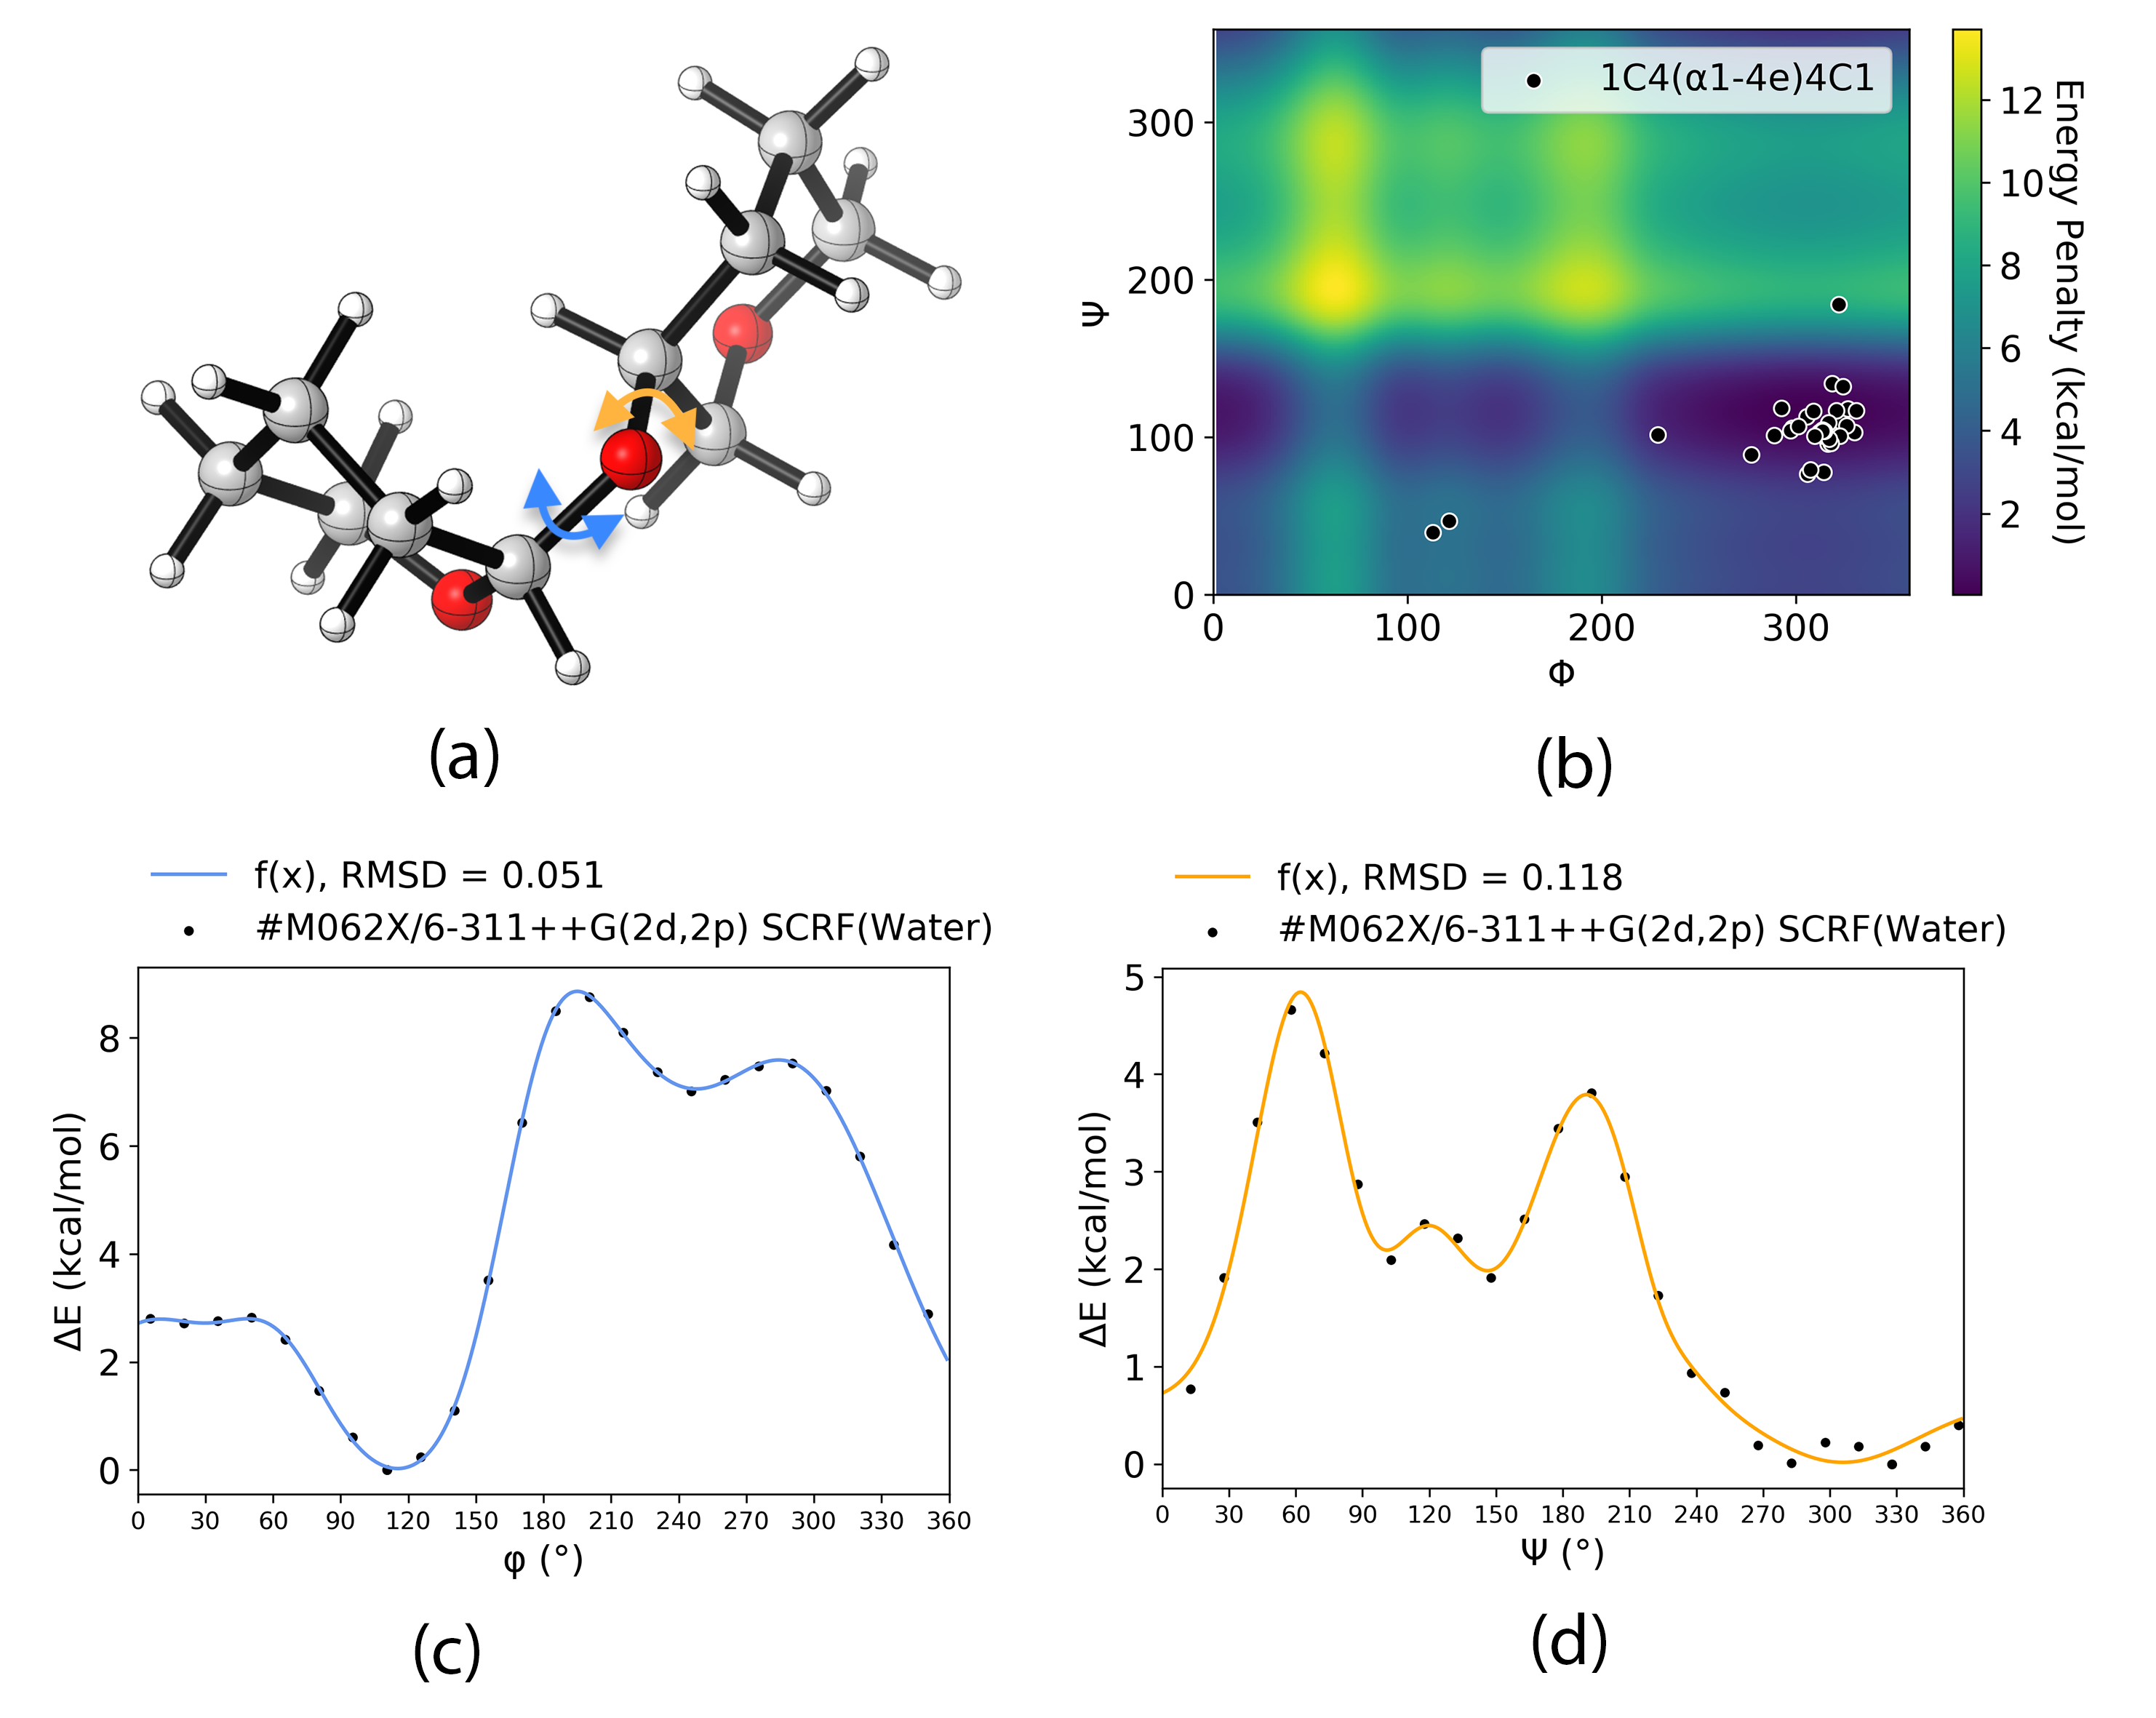
\includegraphics[width=14cm]{Figures/Torsions/La1_4eD.png}
    \caption{}
    \label{fig:1c4_a_e_4c1}
\end{figure}


\section{Saltbridge Energy Scoring Function}
\subsection{Methods}
\subsubsection*{Preparing the model structures}


\subsubsection*{Quantum mechanics calculations}


\subsubsection*{Fitting the Model}

\subsection{Results and Discussion}


\chapter{Benchmarking Docking Software for Glycosaminoglycans}

\section{Methods}
\subsection{Docking}
\noindent \textbf{Structure Preparation}

\noindent \textbf{Docking Protocol}\\
\noindent \textit{Statistical Considerations}\\
In an effort to determine a statistically significant sample size, an initial trial of docking, using the default \ac{VC} parameters (\textit{CHI cutoff} = 0, \textit{CHI coeff} = 1) for a subset of structures containing sugars in a $^{1}C_{4}$ or $^{4}C_{1}$ ring conformation, exclusively. Docking was repeated 36 times, with \ac{ADV} parameters \textit{exhaustiveness} and \textit{energy range} set to 80 and 12, respectively. The top five docked poses produced by \ac{VC} were scored by \ac{RMSD} from the native crystal pose. From these docking calculations, a mean standard error ($E$) of 0.32 \ac{RMSD} and mean standard deviation ($\sigma$) of 0.21 \ac{RMSD} were observed. To produce a statistically significant result (i.e. $p < 0.5, Z = 1.96$), the minimum sample size required can be calculated by:
\begin{equation}  \label{eq:statistical_considerations}
   n_{0} = \Big(\frac{Z \sigma}{E}\Big)^{2} = \Big(\frac{1.96 \times 0.21}{0.32}\Big)^{2} = 9.83 \approx 10 
\end{equation}
\\
\\

\subsection{Analysis}
\section{Results and Discussion}

\subsection{Comparing the Performance of Autodock Vina and Vina-Carb}


\begin{figure}
    \centering
    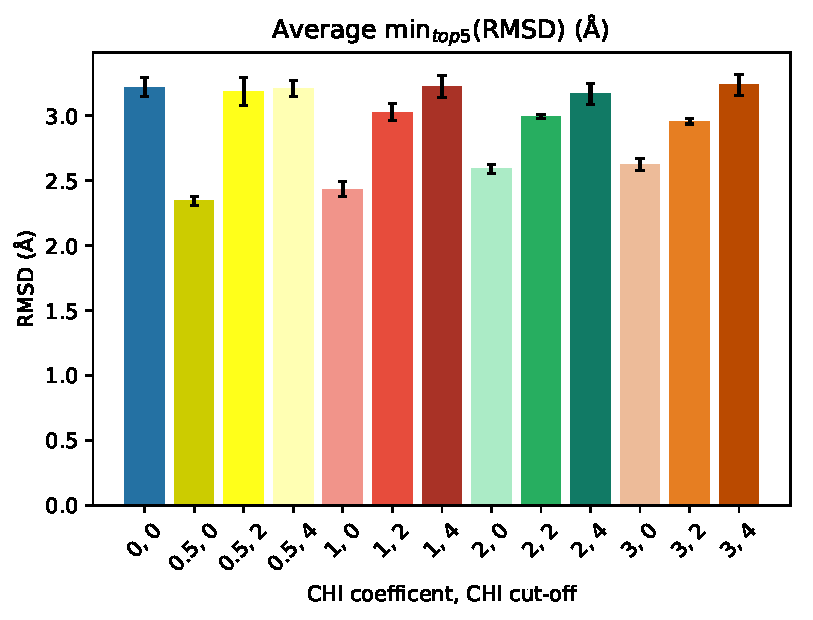
\includegraphics[width=8cm]{Figures/Docking/chairs_RMSD.pdf}
    \caption{Caption}
    \label{fig:my_label}
\end{figure}

\chapter{GlycoTorch Web Server}



\newpage
\setstretch{-1}
\printbibliography

\newpage
\chapter{Appendix A}
\vspace{1cm}

\begin{multline}
f(x) = 13.3370e^{-\frac{(x-31.3775)^{2} } { 16552.6689 } }
1.3170e^{-\frac{(x-135.6499)^{2} } { 391.0353 } } +
2.8463e^{-\frac{(x-160.7422)^{2} } { 226.0367 } } \\ +
0.5915e^{-\frac{(x-314.4487)^{2} } { 328.4058 } }  +
8.8900e^{-\frac{(x-189.8429)^{2} } { 1773.6483 } } +
16.0838e^{-\frac{(x-305.3791)^{2} } { 8985.1546 } } \\ + -9.9028
\quad \quad 0 \leq x < 360
\end{multline}

%%%% un-comment for appendix
% \newpage
% \section{Appendix}


\end{document}

